\section{HÌNH TRỤ} % Tên bài
\subsection{Kiến thức trọng tâm}
\subsubsection{Hình trụ}
\begin{dn}
	Khi quay hình chữ nhật $AA'O'O$ một vòng quanh cạnh $OO'$ cố định ta được một {\it hình trụ}.
	\begin{center}
		\begin{tikzpicture}[>=stealth,line join=round,line cap=round,font=\footnotesize,scale=1]
			\def\a{1.7} % ban truc lon = ban kinh tru
			\def\b{0.6} % ban truc nho
			\def\h{2.6} % chieu cao tru
			\begin{scope}[shift = ({-4,0})]
				\path 
				(0,\h) coordinate (O)
				(0,0) coordinate (O')
				(-\a,\h) coordinate (A)  
				(-\a,0) coordinate (A') 
				($(O)!1.3!(O')$) coordinate (x)
				($(O')!1.3!(O)$) coordinate (y)
				;
				% ve cac canh ben
				\draw (A)--(O)--(O')--(A')--cycle (x)--(y);
				\draw[->] (-0.1,1.3) arc [x radius=0.2, y radius=0.15, start angle=120, end angle=420];
				\foreach \l/\g in {O/0,O'/0,A/135,A'/-135}
				\draw[fill=black] (\l) circle (1pt) +(\g:.3) node{$\l$};
			\end{scope}
			\path 
			(\a,\h) coordinate (M)
			(\a,0) coordinate (Q)
			(0,\h) coordinate (O)
			(0,0) coordinate (O')
			(-\a,\h) coordinate (N) 
			(-\a,0) coordinate (P)
			($(O)!1.3!(O')$) coordinate (x)
			($(O')!1.3!(O)$) coordinate (y)
			(1.2,-0.42) coordinate (A')
			(1.2,2.18) coordinate (A)
			;
			\fill[color=cyan!15] (O)--(A)--(A')--(O')--cycle;
			% ve day duoi
			\draw[dashed] (\a,0) arc [x radius=\a, y radius=\b, start angle=0, end angle=180];
			\draw (-\a,0) arc [x radius=\a, y radius=\b, start angle=180, end angle=360];
			% ve day tren
			\draw (0,\h) ellipse (\a cm and \b cm);
			\draw[dashed] (O')--(O) (O')--(A');
			% ve cac canh ben
			\draw (M)--(Q) (N)--(P) (O)--(x) (O')--(y) (O)--(A)--(A');
			%\draw[dashed] (-\a,0)--(\a,0) (-\a,\h)--(\a,\h);
			\foreach \l/\g in {O/180,O'/180}
			\draw[fill=black] (\l) circle (1pt) +(\g:.3) node{$\l$};
			\draw[fill=black] (A) circle (1pt) +(90:.3) node{$A$};
			\draw[fill=black] (A') circle (1pt) +(-90:.3) node{$A'$};
			\fill ($(O)!0.5!(A)$) node[above]{$r$};
			\fill ($(O')!0.5!(A')$) node[above]{$r$};
			\draw[<->] (-1.9,0)--(-1.9,2.6) node[midway,above,rotate=90]{chiều cao};
			\draw[->] (2.3,2) node[right]{đường sinh}--(1.25,1.3);
			\draw[->] (0.3,-1.3) node[below]{bán kính đáy}--(0.5,-0.3);
		\end{tikzpicture}
	\end{center}
	\begin{itemize}
		\item Cạnh $OA$, $O'A'$ quét thành hai hình tròn có cùng bán kính gọi là {\it hai đáy} của hình trụ; bán kính của đáy được gọi là {\it bán kính đáy} của hình trụ.
		\item Cạnh $AA'$ quét thành mặt xung quanh của hình trụ, mỗi vị trí của $AA'$ được coi là một {\it đường sinh}.
		\item Độ dài đoạn $OO'$ gọi là {\it chiều cao} của hình trụ. Các đường sinh có độ dài bằng nhau và bằng chiều cao của hình trụ.
	\end{itemize}
\end{dn}

\begin{luuy}
	Từ một hình trụ, nếu ta cắt rời hai đáy và cắt theo một đường sinh nào đó rồi trải phẳng ra thì ta được một hình phẳng (gồm hai hình tròn và một hình chữ nhật) như hình bên dưới gọi là \textit{hình khai triển của hình trụ} đã cho.
	\begin{center}
		\begin{tikzpicture}[>=stealth,line join=round,line cap=round,font=\footnotesize,scale=0.9]
			\def\a{0.8} % ban truc lon = ban kinh tru
			\def\b{0.4} % ban truc nho
			\def\h{1.5} % chieu cao tru
			\path 
			(\a,\h) coordinate (A)
			(\a,0) coordinate (B)
			(0,\h) coordinate (O')
			(0,0) coordinate (O);
			\draw[dashed] (O')--(O)--(B);
			% ve cac canh ben
			\draw (\a,0)--(\a,\h) (-\a,0)--(-\a,\h) (O')--(A);
			% ve day duoi
			\draw[dashed] (\a,0) arc [x radius=\a, y radius=\b, start angle=0, end angle=180];
			\draw (-\a,0) arc [x radius=\a, y radius=\b, start angle=180, end angle=360];
			% ve day tren
			%\draw[dashed, thick] (\a,\h) arc [x radius=\a, y radius=\b, start angle=0, end angle=180];
			%\draw[thick] (-\a,\h) arc [x radius=\a, y radius=\b, start angle=180, end angle=360];
			\draw (0,\h) ellipse (\a cm and \b cm);
			%\draw[dashed] (-\a,0)--(\a,0) (-\a,\h)--(\a,\h);
			\foreach \l/\g in {A/0,B/-45}
			\draw[fill=black] (\l) circle (1pt) +(\g:.3) node{$\l$};
			\draw[->] (1.5,0.75)--(2.5,0.75);
			\draw (3,\h)--(3,0)--(8,0)--(8,\h)--cycle;
			\draw[fill=black] (3,\h) circle (1pt) +(180:.3) node{$A$};
			\draw[fill=black] (3,0) circle (1pt) +(-135:.3) node{$B$};
			\draw ($(4.2,\a)+(0,\h)$) ellipse (\a cm and \a cm);
			\draw (6.8,-\a) ellipse (\a cm and \a cm);
			\draw[dashed] (4.2,2.3)--(5,2.3) (6.8,-0.8)--(7.6,-0.8);
		\end{tikzpicture}
	\end{center}
\end{luuy}

\subsubsection{Diện tích xung quanh của hình trụ}
\begin{dn}
	Cho hình trụ có bán kính đáy $r$ và chiều cao $h$. 
	\begin{center}	\begin{tikzpicture}[>=stealth,line join=round,line cap=round,font=\footnotesize,scale=1]
			\def\a{1.5};\def\b{0.3};\def\c{3};
			\draw
			[dashed] (1.8,0) arc(0:180:1.8cm and 0.5cm) % vòng cung khuất dưới
			(0,0)--++(90:\c)node[midway,right]{$h$}--++(0:1.8)node[midway,above]{$r$}
			;
			\draw 
			(-1.8,0) arc(180:360:1.8cm and 0.5cm) % vòng cung nhìn thấy dưới
			($(1.8,0)+(90:\c)$) arc(0:360:1.8cm and 0.5cm)
			(1.8,0)--++(90:\c) (-1.8,0)--++(90:\c)
			;
			\draw (0,\c)node[above]{$O$} 
			(0,0)node[left]{$O'$}
			;
			\foreach \y in {0,\c}{\fill (0,\y) circle (1.5pt);}
	\end{tikzpicture}\end{center}
	Khi đó 
	\begin{itemize}
		\item Diện tích xung quanh $S_{\text{xq}}=2\pi rh$.
		\item Diện tích toàn phần bằng tổng diện tích xung quanh và diện tích hai đáy
		$$S_{\text{tp}}=2\pi rh+2\pi r^2.$$
	\end{itemize}
\end{dn}

\subsubsection{Thể tích của hình trụ}
\begin{dn}
	Thể tích $V$ của hình trụ có bán kính đáy $r$ và chiều cao $h$ là
	$$V=S\cdot h=\pi r^2h\ (S\text{ là diện tích đáy của hình trụ}).$$
	\begin{center}	\begin{tikzpicture}[>=stealth,line join=round,line cap=round,font=\footnotesize,scale=1]
			\def\a{1.5};\def\b{0.3};\def\c{3};
			\draw
			[dashed] (1.8,0) arc(0:180:1.8cm and 0.5cm) % vòng cung khuất dưới
			(0,0)--++(90:\c)node[midway,right]{$h$}--++(0:1.8)node[midway,above]{$r$}
			;
			\draw 
			(-1.8,0) arc(180:360:1.8cm and 0.5cm) % vòng cung nhìn thấy dưới
			($(1.8,0)+(90:\c)$) arc(0:360:1.8cm and 0.5cm)
			(1.8,0)--++(90:\c) (-1.8,0)--++(90:\c)
			;
			\draw (0,\c)node[above]{$O$} 
			(0,0)node[left]{$O'$}
			;
			\foreach \y in {0,\c}{\fill (0,\y) circle (1.5pt);}
	\end{tikzpicture}\end{center}
\end{dn}

\begin{vd}%[Dự án EX-9-Đề Cương Toán 9]%[Đặng Thị Lâm]%[9H4N1-1]
	Quan sát và cho biết bán kính đáy, đường sinh, độ dài đường sinh và chiều cao của hình trụ trong các hình bên dưới.
	\begin{center}
		\begin{tikzpicture}[>=stealth,line join=round,line cap=round,font=\footnotesize,scale=1]
			\def\a{1.5};\def\b{0.3};\def\c{4};
			\draw
			[dashed] (1.8,0) arc(0:180:1.8cm and 0.5cm) % vòng cung khuất dưới
			(0,0)--++(90:\c)--++(0:1.8)
			;
			\fill (1.8,4) circle(1pt) node[right]{$A$};
			\fill (1.8,0) circle(1pt) node[right]{$A'$};
			\draw 
			(-1.8,0) arc(180:360:1.8cm and 0.5cm) % vòng cung nhìn thấy dưới
			($(1.8,0)+(90:\c)$) arc(0:360:1.8cm and 0.5cm)
			(1.8,0)--++(90:\c) (-1.8,0)--++(90:\c)node[midway,left]{$h$}
			;
			\draw (0,\c)node[left]{$O$} 
			(0,0)node[left]{$O'$}
			;
			\draw[dashed] (0,0)--(1.5,0)node[midway,sloped,fill=white]{$r$};
			\foreach \y in {0,\c}{\fill (0,\y) circle (1.5pt);}
			\fill (0,-1) node[below]{a)};
			\begin{scope}[shift = ({6,0})]
				\def\a{1.5};\def\b{0.3};\def\c{4};
				\draw
				[dashed] (1.8,0) arc(0:180:1.8cm and 0.5cm) % vòng cung khuất dưới
				(0,0)--++(90:\c)--++(0:1.8)
				;
				\fill (1.8,4) circle(1pt) node[right]{$A$};
				\fill (1.8,0) circle(1pt) node[right]{$B$};
				\draw 
				(-1.8,0) arc(180:360:1.8cm and 0.5cm) % vòng cung nhìn thấy dưới
				($(1.8,0)+(90:\c)$) arc(0:360:1.8cm and 0.5cm)
				(1.8,0)--++(90:\c)node[midway,right]{$6$ cm} (-1.8,0)--++(90:\c)
				;
				\draw (0,\c)node[left]{$O$} 
				(0,0)node[left]{$O'$}
				;
				\draw[dashed] (0,0)--(1.5,0);
				\fill (0.75,0) node[above]{$2$ cm};
				\foreach \y in {0,\c}{\fill (0,\y) circle (1.5pt);}
				\fill (0,-1) node[below]{b)};
			\end{scope}
		\end{tikzpicture}
	\end{center}
	\loigiai{
		\begin{itemize}
			\item Hình trụ a) có bán kính là $r$; đường sinh là $AA'$; $h$ là độ dài đường sinh và cũng là chiều cao của hình trụ đó.
			\item Hình trụ b) có bán kính là $r=2$ cm; đường sinh là $AB = 6$ cm; $h=6$ cm là độ dài đường sinh và cũng là chiều cao của hình trụ đó.
		\end{itemize}
	}
\end{vd}

\begin{vd}%[Dự án EX-9-Đề Cương Toán 9]%[Đặng Thị Lâm]%[9H4N1-2]%[9H4N1-3]
	Tính diện tích xung quanh, diện tích toàn phần và thể tích của hình trụ có bán kính đáy $2$ m và chiều cao $3$ m.
	\loigiai
	{
		Theo đề bài, hình trụ có có bán kính đáy $r=2$ m và chiều cao $h=3$ m.\\
		Diện tích xung quanh của hình trụ là 
		$$S_{\text{xq}}=2\pi rh=2\pi\cdot2\cdot3=12\pi\text{ (m$^2$).}$$
		Diện tích toàn phần của hình trụ là 
		$$S_{\text{tp}}=2\pi rh + 2\pi r^2 = 2\pi\cdot2\cdot3 + 2\pi\cdot2^2 = 20\pi\text{ (m$^2$).}$$
		Thể tích của hình trụ là
		$$V=\pi r^2h=\pi\cdot2^2\cdot3=12\pi\text{ (m$^3$).}$$
	}
\end{vd}

\begin{vd}%[Dự án EX-9-Đề Cương Toán 9]%[Đặng Thị Lâm]%[9H4N1-2]%[9H4H1-1]
	Tạo lập chiếc hộp dạng hình trụ có chiều cao $10$ cm, bán kính đáy $3$ cm.
	\loigiai{ 
		\begin{itemize}
			\item Bước 1: Cắt một tấm bìa hình chữ nhật có cạnh $10$ cm và cạnh $6\pi$ cm $\approx19$ cm.
			\item Bước 2: Ghép hai cạnh $10$ cm của tấm bìa lại với nhau sao cho hai cạnh $6\pi$ cm được uốn cong tạo thành hai đường tròn.
			\item Bước 3: Cắt hai tấm bìa hình tròn bán kính $3$ cm rồi dán vào hai hình tròn vừa tạo thành, ta được chiếc hộp như yêu cầu.
		\end{itemize}
	}
\end{vd}

\begin{vd}%[Dự án EX-9-Đề Cương Toán 9]%[Đặng Thị Lâm]%[9H4V1-4]
	Một nhà máy dự định sản xuất thùng phuy đựng dầu nhớt dạng hình trụ có đường kính đáy $0{,}6$ m và chiều cao $0{,}9$ m. Bỏ qua diện tích các mép thùng, hãy tính diện tích thép cần để sản xuất $100$ thùng phuy như vậy (\textit{kết quả làm tròn đến hàng phần trăm}).
	\loigiai{
		Bán kính đáy của thùng phuy là $0{,}6:2 = 0{,}3$ (m).\\
		Diện tích thép để sản xuất $1$ thùng phuy chính là diện tích toàn phần của hình trụ do đó
		$$S_{\text{tp}}=2\pi rh+2\pi r^2=2\pi\cdot0{,}3\cdot0{,}9 + 2\cdot0{,}3^2\pi = 0{,}72\pi \text{ (m$^2$).}$$
		Như vậy khi sản xuất $100$ thùng phuy ta cần số thép là
		$$100\cdot0{,}72\pi = 72\pi \approx 226{,}19\text{ (m$^2$).}$$
	}
\end{vd}

\subsection{BÀI TẬP}

\begin{bt}%[Dự án EX-9-Đề Cương Toán 9]%[Đặng Thị Lâm]%[9H4N1-1]
	Trong các hình sau đây, hình nào là hình trụ?
	\begin{center}
		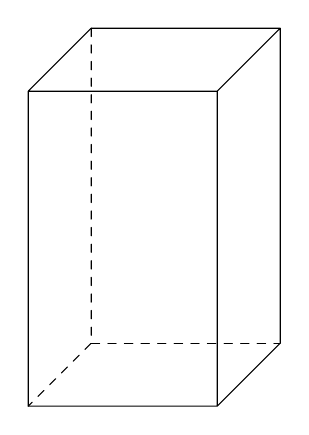
\begin{tikzpicture}[>=stealth,line join=round,line cap=round,font=\footnotesize,scale=0.8]
			\draw (3,0)--(0,0)--(0,-5)--(3,-5)--(4,-4)--(4,1)--(1,1)--(0,0) (3,-5)--(3,0)--(4,1);
			\draw [dashed] (1,1)--(1,-4)--(0,-5);
			\draw [dashed] (1,-4)--(4,-4);
		\end{tikzpicture}
		\hspace{1cm}
		\begin{tikzpicture}[>=stealth,line join=round,line cap=round,font=\footnotesize,scale=0.8]
			\def\a{1.5};\def\b{0.3};\def\c{3};
			\draw
			[dashed](1.8,0) arc(0:180:1.8cm and 0.5cm) % vòng cung khuất dưới
			;
			\draw 
			(-1.8,0) arc(180:360:1.8cm and 0.5cm) % vòng cung nhìn thấy dưới
			($(1.8,0)+(90:\c)$) arc(0:360:1.8cm and 0.5cm)
			(1.8,0)--++(90:\c) (-1.8,0)--++(90:\c)
			;
			\foreach \y in {0,\c}{\fill (0,\y) circle (1pt);}
		\end{tikzpicture}
		\hspace{1cm}
		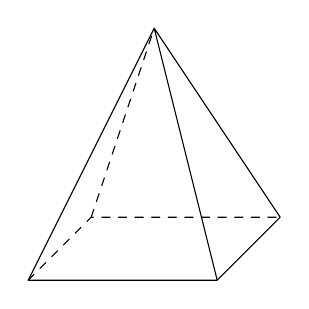
\begin{tikzpicture}[>=stealth,line join=round,line cap=round,font=\footnotesize,scale=0.8]
			\draw (0,0)--(3,0)--(4,1)--(2,4)--(3,0) (2,4)--(0,0);
			\draw [dashed] (0,0)--(1,1)--(4,1);
			\draw [dashed] (1,1)--(2,4);
		\end{tikzpicture}
		\hspace{1cm}
		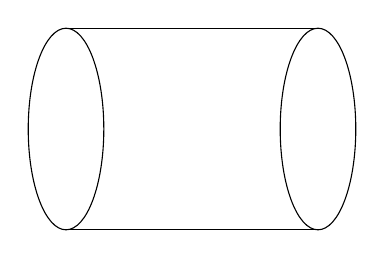
\begin{tikzpicture}[>=stealth,line join=round,line cap=round,font=\footnotesize,scale=0.8]
			\def\a{0.6};\def\b{1.6};\def\c{4};
			\draw(0,0) ellipse (\a cm and \b cm)
			;
			\draw	(0,\b)--++(0:\c);
			\draw  (0,-\b)--++(0:\c);
			\draw (4,0) ellipse (\a cm and \b cm) ;
		\end{tikzpicture}
	\end{center}
	\loigiai{
		Hình 2 và hình 4 (từ trái sang) là hình trụ.
	}
\end{bt}

\begin{bt}%[Dự án EX-9-Đề Cương Toán 9]%[Đặng Thị Lâm]%[9H4N1-1]
	Trong những vật thể ở các hình $a$, $b$, $c$, $d$, $e$, vật thể nào có dạng hình trụ?
	\begin{center}
		\begin{tikzpicture}[line join=round,line cap=round,font=\footnotesize,scale=1]
			\def \canh{2}
			\path 
			(0:0) coordinate (D')
			+(90:\canh) coordinate (D)
			+(0:\canh) coordinate (C')
			+(40:.6*\canh) coordinate (A')
			($(C')+(D)-(D')$) coordinate (C)
			($(D)+(A')-(D')$) coordinate (A)
			($(C')+(A')-(D')$) coordinate (B')
			($(C)+(A)-(D)$) coordinate (B)
			;
			\draw[dashed] 
			(A')--(A) (A')--(B') (A')--(D')
			;
			\draw 
			(A)--(B)--(B')--(C')--(D')--(D)--cycle
			(C)--(B) (C)--(D) (C)--(C')
			;
			\foreach \x/\g in {D'/-90,C'/-90,D/180,A'/135,C/-45,A/90,B'/0,B/90}
			\fill (\x) circle (1pt)
			+(\g:3mm) node {};
			\path ($(current bounding box.south)+(0,-.5)$) node {Hình $a$};
			
		\end{tikzpicture} \hspace{.2cm}
		\begin{tikzpicture}[scale=1,x=1cm,y=1cm,line join=round,line cap=round,font=\footnotesize] 
			\def\x{1.5}  %bán trục lớn elip1 
			\def\y{.5}  %bán trục bé elip 
			\path 
			(0:0) coordinate (O)
			+(180:\x) coordinate (A)
			+(0:\x) coordinate (B)
			;
			
			\draw[dashed] 
			(B) arc (0:180:{\x} and {\y})
			;
			\draw 
			(O) circle (\x)
			(B) arc (0:-180:{\x} and {\y})
			;
			\foreach \x/\g in {O/-90}
			\fill (\x) circle (1pt)
			+(\g:3mm) node {};
			\path ($(current bounding box.south)+(0,-.5)$) node {Hình $b$};
		\end{tikzpicture}\hspace{.2cm}
		\begin{tikzpicture}[scale=1,font=\footnotesize,>=stealth]%<DTools>
			%Gán số liệu.
			\def\canhAC{2};\def\canhBA{1};\def\gocBAC{-50};\def\h{2};
			%Gán tọa độ.
			\coordinate (A) at (0,0);
			\coordinate (B) at ($(A)+(\gocBAC:\canhBA)$);
			\coordinate (C) at ($(A)+(0:\canhAC)$);
			\coordinate (O) at ($1/3*(A)+1/3*(B)+1/3*(C)$);
			\coordinate (S) at ($(O)+(90:\h)$);
			%Vẽ khối chóp S.ABC đều.
			\draw (S)--(B) (S)--(A)--(B) (S)--(C)--(B);
			\draw[dashed] (A)--(C);
			%Gán nhãn.
			\foreach \x/\y in {S/90,A/180,B/-90,C/0}{\fill (\x) circle (1pt) ($(\x)+(\y:0.3cm)$) node{};}
			\path ($(current bounding box.south)+(0,-.5)$) node {Hình $c$};
		\end{tikzpicture}\hspace{.2cm}
		\begin{tikzpicture}[line
			join=round,line
			cap=round,font=\footnotesize]
			\def\a{1}
			\def\b{.3}
			\def\h{2}
			\pgfmathsetmacro\g{asin(\b/\h)}
			\pgfmathsetmacro\xo{\a*cos(\g)}
			\pgfmathsetmacro\yo{\b*sin(\g)}
			\path
			(0,0) coordinate (O) %Tâm của đáy nón
			+(90:\h) coordinate (S) %Đỉnh của nón
			+(180:\a) coordinate (A) %Đỉnh trai của elip
			+(0:\a) coordinate (B) %Đỉnh phải của elip
			(\xo,\yo) coordinate (M) %Chân đường sinh phải
			(-\xo,\yo) coordinate (N) %Chân đường sinh trái
			;
			\draw[dashed]
			(M) arc (\g:180-\g:{\a} and
			{\b})
			;
			\draw (S)--(N) arc
			(180-\g:360+\g:{\a} and
			{\b})--cycle;
			\foreach \x/\g in {S/90}
			\fill (\x) circle (1pt)+(\g:3mm) node{};
			\path ($(current bounding box.south)+(0,-.5)$) node {Hình $d$};
			
		\end{tikzpicture}\hspace{.2cm}
		\begin{tikzpicture}[scale=1,font=\footnotesize,>=stealth]%<DTools>
			%Gán số liệu.
			\def\a{1};\def\b{0.5};\def\h{2};
			%Gán tọa độ.
			\coordinate (O) at (0,0);
			\coordinate (O') at ($(O)+(90:\h)$);
			\coordinate (B') at ($(O)-(0:\a)$);
			\coordinate (B) at ($(O)+(0:\a)$);
			\coordinate (A') at ($(B')+(90:\h)$);
			\coordinate (A) at ($(B)+(90:\h)$);
			%Vẽ khối trụ.
			\draw (B) arc (0:-180:\a cm and \b cm) (A) arc (0:360:\a cm and \b cm) (B')--(A') (B)--(A);
			\draw[dashed] (B) arc (0:180:\a cm and \b cm);
			\path ($(current bounding box.south)+(0,-.5)$) node {Hình $e$};
			
		\end{tikzpicture}
	\end{center}
	\loigiai{
		Trong các vật thể ở các hình $a$, $b$, $c$, $d$, $e$, vật thể ở hình $e$ có dạng hình trụ.
	}
\end{bt}

\begin{bt}%[Dự án EX-9-Đề Cương Toán 9]%[Đặng Thị Lâm]%[9H4N1-1]
	Trong những vật thể ở các hình $a$, $b$, $c$, $d$, vật thể ở hình nào có dạng hình trụ?
	\begin{center}
	\begin{tikzpicture}[scale=1, font=\footnotesize,>=stealth]%<DTools>
		%Gán số liệu.
		\def\a{1};\def\b{0.5};\def\h{2};
		%Gán tọa độ.
		\coordinate (O) at (0,0);
		\coordinate (O') at ($(O)+(90:\h)$);
		\coordinate (B') at ($(O)-(0:\a)$);
		\coordinate (B) at ($(O)+(0:\a)$);
		\coordinate (A') at ($(B')+(90:\h)$);
		\coordinate (A) at ($(B)+(90:\h)$);
		%Vẽ khối trụ.
		\draw (B) arc (0:-180:\a cm and \b cm) (A) arc (0:360:\a cm and \b cm) (B')--(A') (B)--(A);
		\draw[dashed] (B) arc (0:180:\a cm and \b cm);
		\path ($(current bounding box.south)+(0,-.5)$) node {Hình $a$};
	\end{tikzpicture}\hspace{1cm}
	\begin{tikzpicture}[scale=1, font=\footnotesize,>=stealth]%<DTools>
		%Gán số liệu.
		\def\a{1};\def\b{0.5};\def\h{2};
		%Gán tọa độ.
		\coordinate (O) at (0,0);
		\coordinate (O') at ($(O)+(90:\h)$);
		\coordinate (B') at ($(O)-(0:\a)$);
		\coordinate (B) at ($(O)+(0:\a)$);
		\coordinate (A') at ($(B')+(90:\h-.5)$);
		\coordinate (A) at ($(B)+(90:\h)$);
		%Vẽ khối trụ.
		\draw (B) arc (0:-180:\a cm and \b cm) (B')--(A') (B)--(A);
		\draw[dashed] (B) arc (0:180:\a cm and \b cm);
		\draw[smooth] (A') .. controls ++(-90:.6) and ++(-90:.4) .. (A) .. controls ++(90:.6) and ++(90:.4) .. (A');
		
		
		\foreach \x/\g in {A/90,A'/0}\fill (\x) circle (0pt)+(\g:3mm) node{};
		\path ($(current bounding box.south)+(0,-.5)$) node {Hình $b$};
		
	\end{tikzpicture}\hspace{1cm}
	\begin{tikzpicture}[scale=1, font=\footnotesize,>=stealth]
		%Gán số liệu.
		\def\a{1};\def\b{0.5};\def\h{2};
		%Gán tọa độ.
		\coordinate (O) at (0,0);
		\coordinate (O') at ($(O)+(90:\h)$);
		\coordinate (B') at ($(O)-(0:\a)$);
		\coordinate (B) at ($(O)+(0:\a)$);
		\coordinate (A') at ($(B')+(90:\h)$);
		\coordinate (A) at ($(B)+(90:\h)$);
		%Vẽ khối trụ.
		\draw (B) arc (0:-180:\a cm and \b cm) (A) arc (0:360:\a cm and \b cm);
		\draw (B) to[bend left = -10] (A);
		\draw (B') to[bend left = 10] (A');
		\draw[dashed] (B) arc (0:180:\a cm and \b cm);
		\path ($(current bounding box.south)+(0,-.5)$) node {Hình $c$};
	\end{tikzpicture}
	\begin{tikzpicture}[scale=1, font=\footnotesize,>=stealth]
		\def\a{1.5} 
		\def\b{.3}
		\def\h{-4}
		\pgfmathsetmacro\g{asin(\b/\h)}
		\pgfmathsetmacro\xo{\a *cos(\g)}
		\pgfmathsetmacro\yo{\b *sin(\g)}
		
		\clip (-2.4,-3) rectangle (2,1);
		\path
		(0,0) coordinate (O)
		+(-90:2) coordinate (O') 
		(0,\h) coordinate (S)
		(180:\a) coordinate (A)
		(0:\a) coordinate (B)
		(-\xo,\yo) coordinate (A1) %Tọa độ tiếp điểm trái
		(\xo,\yo) coordinate (B1) %Tọa độ tiếp điểm phải
		($(S)!.5!(A1)$) coordinate (A2)
		($(S)!.5!(A)$) coordinate (A') %Đỉnh elip đáy
		($(S)!.5!(B1)$) coordinate (B2)
		($(S)!.5!(B)$) coordinate (B') %Đỉnh elip đáy
		%($(A')!.5!(B')$) coordinate (O') 
		;
		\path ($(O')+(0,-.7)$) node {Hình $d$};
		%Đáy nhỏ
		\draw[dashed] (B2) arc (\g:180+\g:{.75} and {.15});
		\draw (B2) arc (\g:-180:{.75} and {.15});
		%Đáy lớn
		\draw (\xo,\yo) arc (\g:360+\g:{\a} and {\b});
		%Đường sinh nón cụt
		\draw (B1)--(B2) (A1)--(A2);
		
		\foreach \x/\g in {S/-90,O/90,A/180,B/0,O'/0} 
		\fill[black] (\x) circle (0pt) ($(\x)+(\g:3mm)$) node{};
	\end{tikzpicture}
\end{center}
\loigiai{
	Trong các vật thể ở các hình $a$, $b$, $c$, $d$, vật thể ở hình $a$ có dạng hình trụ.
}
\end{bt}
\begin{bt}%[Dự án EX-9-Đề Cương Toán 9]%[Đặng Thị Lâm]%[9H4H1-1]
	Cho hình chữ nhật $ABCD$, các điểm $O$, $I$ lần lượt là trung điểm các cạnh $AD$, $BC$. Xét hình trụ được tạo ra khi quay hình chữ nhật $AOIB$ một vòng xung quanh đường thẳng cố định chứa cạnh $OI$ của hình chữ nhật đó (Hình vẽ). Quan sát hình vẽ, hãy chỉ ra
	\begin{center}
		\begin{tikzpicture}[scale=1, font=\footnotesize,>=stealth]%<DTools>
			%Gán số liệu.
			\def\a{2};\def\b{0.5};\def\h{3};
			%Gán tọa độ.
			\coordinate (O) at (0,0);
			\coordinate (O') at ($(O)+(90:\h)$);
			\coordinate (1) at ($(O)-(0:\a)$);
			\coordinate (2) at ($(O)+(0:\a)$);
			\coordinate (3) at ($(1)+(90:\h)$);
			\coordinate (4) at ($(2)+(90:\h)$);
			\path ($(O)+(45:{\a} and {\b})$) coordinate (C)
			($(O)+(-135:{\a} and {\b})$) coordinate (B)
			($(O)+(-90:{\a} and {\b})$) coordinate (6)
			($(O')+(45:{\a} and {\b})$) coordinate (D)
			($(O')+(-135:{\a} and {\b})$) coordinate (A)
			(O')+(90:1) coordinate (5)
			(O)+(90:-1) coordinate (7)
			;
			\draw (B)--(A)--(D);
			%Vẽ khối trụ.
			\draw (2) arc (0:-180:\a cm and \b cm) (4) arc (0:360:\a cm and \b cm) (1)--(3) (2)--(4)  (O')--(5)  (6)--(7);
			\draw[dashed] (2) arc (0:180:\a cm and \b cm) (O)--(O')
			(B)--(C)--(D) (O)--(6)
			;
			%Gán nhãn.
			\foreach \x/\y in {C/45,B/-135,A/-135,D/45}{\fill (\x) circle(1pt) ($(\x)+(\y:0.3cm)$) node{$\x$};}
			\fill
			(O') circle (1.5pt) node[above right] {$O$}
			(O) circle (1.5pt) node[below right] {$I$}
			;
		\end{tikzpicture}
	\end{center}
	\begin{enumerate}
		\item Bốn bán kính đáy của hình trụ;
		\item Chiều cao của hình trụ;
		\item Hai đường sinh của hình trụ. 
	\end{enumerate}
	\loigiai{
		\begin{enumerate}
			\item Bốn bán kính đáy của hình trụ là $IB$; $IC$; $OA$; $OD$.
			\item Chiều cao của hình trụ là $OI$.
			\item Hai đường sinh của hình trụ là $AB$ và $CD$.
		\end{enumerate}
	}
\end{bt}

\begin{bt}%[Dự án EX-9-Đề Cương Toán 9]%[Đặng Thị Lâm]%[9H4H1-1]
	Cho hình trụ có chiều cao $10$ cm, đường kính đáy $7$ cm (Hình 5a) và hình khai triển của hình trụ đó (Hình 5b). Hãy viết số thích hợp vào mỗi dấu ? trong hình vẽ.
	\begin{center}
		\begin{tikzpicture}[>=stealth,line join=round,line cap=round,font=\footnotesize,scale=1]
			\def\a{1.1} % ban truc lon = ban kinh tru
			\def\b{0.5} % ban truc nho
			\def\h{2.6} % chieu cao tru
			\path 
			(\a,\h) coordinate (A)
			(\a,0) coordinate (B)
			(0,\h) coordinate (O')
			(0,0) coordinate (O);
			% ve cac canh ben
			\draw (\a,0)--(\a,\h) (-\a,0)--(-\a,\h);
			\draw[dashed] (O)--(O') node[midway,right]{$10$ cm};
			\draw[dashed] (-\a,0)--(B);
			\fill (O') circle(1pt);
			\fill (O) circle(1pt);
			% ve day duoi
			\draw[dashed] (\a,0) arc [x radius=\a, y radius=\b, start angle=0, end angle=180];
			\draw (-\a,0) arc [x radius=\a, y radius=\b, start angle=180, end angle=360];
			\draw (0,\h) ellipse (\a cm and \b cm);
			\fill (0,0) node[below]{$7$ cm};
			\fill (0,-1.1) node[below]{a)};
			\begin{scope}[shift = ({3,0})]
				\draw (5,0)--(0,0)--(0,2.6)--(5,2.6)--cycle;
				\draw (1.1,3.7) ellipse (1.1 cm and 1.1 cm);
				\draw (3.9,-1.1) ellipse (1.1 cm and 1.1 cm);
				\draw[dashed] (0,3.7)--(2.2,3.7) (2.8,-1.1)--(5,-1.1);
				\fill (1.1,3.7) circle(1pt);
				\fill (3.9,-1.1) circle(1pt);
				\fill (5,0)--(5,2.6) node[midway,right]{? cm};
				\fill (1.1,3.7) node[above]{? cm};
				\fill (3.9,-1.1) node[above]{? cm};
				\fill (2,-1.1) node[below]{b)};
			\end{scope}
			\fill (3,-1.9) node[below]{\textit{Hình 5}};
		\end{tikzpicture}
	\end{center}
	\loigiai{
		\begin{center}
			\begin{tikzpicture}[>=stealth,line join=round,line cap=round,font=\footnotesize,scale=1]
				\def\a{1.1} % ban truc lon = ban kinh tru
				\def\b{0.5} % ban truc nho
				\def\h{2.6} % chieu cao tru
				\path 
				(\a,\h) coordinate (A)
				(\a,0) coordinate (B)
				(0,\h) coordinate (O')
				(0,0) coordinate (O);
				% ve cac canh ben
				\draw (\a,0)--(\a,\h) (-\a,0)--(-\a,\h);
				\draw[dashed] (O)--(O') node[midway,right]{$10$ cm};
				\draw[dashed] (-\a,0)--(B);
				\fill (O') circle(1pt);
				\fill (O) circle(1pt);
				% ve day duoi
				\draw[dashed] (\a,0) arc [x radius=\a, y radius=\b, start angle=0, end angle=180];
				\draw (-\a,0) arc [x radius=\a, y radius=\b, start angle=180, end angle=360];
				\draw (0,\h) ellipse (\a cm and \b cm);
				\fill (0,0) node[below]{$7$ cm};
				\fill (0,-1.1) node[below]{a)};
				\begin{scope}[shift = ({3,0})]
					\draw (5,0)--(0,0)--(0,2.6)--(5,2.6)--cycle;
					\draw (1.1,3.7) ellipse (1.1 cm and 1.1 cm);
					\draw (3.9,-1.1) ellipse (1.1 cm and 1.1 cm);
					\draw[dashed] (0,3.7)--(2.2,3.7) (2.8,-1.1)--(5,-1.1);
					\fill (1.1,3.7) circle(1pt);
					\fill (3.9,-1.1) circle(1pt);
					\fill (5,0)--(5,2.6) node[midway,right]{$10$ cm};
					\fill (1.1,3.7) node[above]{$7$ cm};
					\fill (3.9,-1.1) node[above]{$7$ cm};
					\fill (2,-1.1) node[below]{b)};
				\end{scope}
			\end{tikzpicture}
		\end{center}
	}
\end{bt}

\begin{bt}%[Dự án EX-9-Đề Cương Toán 9]%[Đặng Thị Lâm]%[9H4H1-3]
	Cho hình bên dưới. Thay dấu \lq\lq?\rq\rq\, bằng giá trị thích hợp và hoàn thành bảng sau vào vở
	\begin{center}
		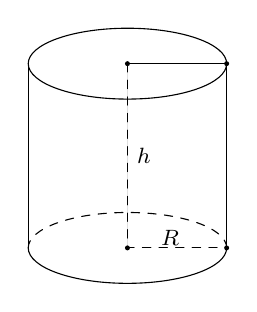
\begin{tikzpicture}[>=stealth,line join=round,line cap=round,font=\footnotesize,scale=0.9]
			\def\a{1.4} % ban truc lon = ban kinh tru
			\def\b{0.5} % ban truc nho
			\def\h{2.6} % chieu cao tru
			\path 
			(\a,\h) coordinate (A)
			(\a,0) coordinate (B)
			(0,\h) coordinate (O')
			(0,0) coordinate (O);
			\draw[dashed] (O')--(O)--(B);
			% ve cac canh ben
			\draw (\a,0)--(\a,\h) (-\a,0)--(-\a,\h) (O')--(A);
			% ve day duoi
			\draw[dashed] (\a,0) arc [x radius=\a, y radius=\b, start angle=0, end angle=180];
			\draw (-\a,0) arc [x radius=\a, y radius=\b, start angle=180, end angle=360];
			\draw (0,\h) ellipse (\a cm and \b cm);
			\fill (O) circle (1pt);
			\fill (O') circle (1pt);
			\fill (A) circle (1pt);
			\fill (B) circle (1pt);
			\fill (O')--(O)node[midway,right]{$h$};
			\fill (0.6,-0.1) node[above]{$R$};
		\end{tikzpicture}
	\end{center}
	\begin{center}
		\begin{tabular}{|c|c|c|c|}
			\hline
			Bán kính đáy (cm) & Chiều cao (cm) & Diện tích xung quanh (cm$^2$) & Thể tích (cm$^3$)\\
			\hline
			$4$ & $6$ & ? & ? \\
			\hline
			$3$ & $5$ & ? & ? \\
			\hline
			? & $10$ & ? & $50\pi$\\
			\hline
			$8$ & ? & $192\pi$ & ? \\
			\hline
		\end{tabular}
	\end{center}
	\loigiai{
		\begin{center}
			\begin{tabular}{|c|c|c|c|}
				\hline
				Bán kính đáy (cm) & Chiều cao (cm) & Diện tích xung quanh (cm$^2$) & Thể tích (cm$^3$)\\
				\hline
				$4$ & $6$ & $48\pi$ & $96\pi$ \\
				\hline
				$3$ & $5$ & $30\pi$ & $45\pi$ \\
				\hline
				$\sqrt{5}$ & $10$ & $20\sqrt{5}\pi$ & $50\pi$\\
				\hline
				$8$ & $12$ & $192\pi$ & $768\pi$ \\
				\hline
			\end{tabular}
		\end{center}
	}
\end{bt}

\begin{bt}%[Dự án EX-9-Đề Cương Toán 9]%[Đặng Thị Lâm]%[9H4N1-3]
	Tìm chiều cao, bán kính đáy và diện tích xung quanh, thể tích của mỗi hình trụ sau
	\begin{center}
		\begin{tikzpicture}[>=stealth,line join=round,line cap=round,font=\footnotesize,scale=1]
			\def\a{1.5};\def\b{0.3};\def\c{4};
			\draw
			[dashed] (1.8,0) arc(0:180:1.8 cm and 0.5 cm) % vòng cung khuất dưới
			(0,0)--++(90:\c)node[midway,right]{\scriptsize $10$ cm}--++(0:1.8)node[midway,sloped,fill=white]{\scriptsize $2$ cm}
			;
			\draw 
			(-1.8,0) arc(180:360:1.8 cm and 0.5 cm) % vòng cung nhìn thấy dưới
			($(1.8,0)+(90:\c)$) arc(0:360:1.8 cm and 0.5 cm)
			(1.8,0)--++(90:\c) (-1.8,0)--++(90:\c)
			;
			\draw (0,\c)node[above]{$O$} 
			(0,0)node[left]{$O'$}
			;
			\foreach \y in {0,\c}{\fill (0,\y) circle (1.5pt);}
			\path ($(current bounding box.south)+(0,-.5)$) node {Hình a)};
		\end{tikzpicture}
		\hspace{1cm}
		\begin{tikzpicture}[>=stealth,line join=round,line cap=round,font=\footnotesize,scale=1]
			\def\a{1.5};\def\b{0.3};\def\c{3};
			\draw
			[dashed] (1.8,0) arc(0:180:1.8 cm and 0.5 cm) % vòng cung khuất dưới
			(0,0)--++(90:\c)node[midway,right]{\scriptsize $8$ cm}--++(0:1.8)node[midway,sloped,fill=white]{\scriptsize $4$ cm}
			;
			\draw 
			(-1.8,0) arc(180:360:1.8 cm and 0.5 cm) % vòng cung nhìn thấy dưới
			($(1.8,0)+(90:\c)$) arc(0:360:1.8 cm and 0.5 cm)
			(1.8,0)--++(90:\c) (-1.8,0)--++(90:\c)
			;
			\draw (0,\c)node[above]{$O$} 
			(0,0)node[left]{$O'$}
			;
			\foreach \y in {0,\c}{\fill (0,\y) circle (1.5pt);}
			\path ($(current bounding box.south)+(0,-.5)$) node {Hình b)};
		\end{tikzpicture}
		\hspace{1cm}
		\begin{tikzpicture}[>=stealth,line join=round,line cap=round,font=\footnotesize,scale=1]
			\def\a{1.5};\def\b{0.3};\def\c{2.5};
			\draw
			[dashed] (1.8,0) arc(0:180:1.8 cm and 0.5 cm) % vòng cung khuất dưới
			(0,0)--++(90:\c)node[midway,right]{\scriptsize $7$ cm}--++(0:1.8)node[midway,sloped,fill=white]{\scriptsize $3$ cm}
			;
			\draw 
			(-1.8,0) arc(180:360:1.8 cm and 0.5 cm) % vòng cung nhìn thấy dưới
			($(1.8,0)+(90:\c)$) arc(0:360:1.8 cm and 0.5 cm)
			(1.8,0)--++(90:\c) (-1.8,0)--++(90:\c)
			;
			\draw (0,\c)node[above]{$O$} 
			(0,0)node[left]{$O'$}
			;
			\foreach \y in {0,\c}{\fill (0,\y) circle (1.5pt);}
			\path ($(current bounding box.south)+(0,-.5)$) node {Hình c)};
		\end{tikzpicture}
	\end{center}
	\loigiai{
		\begin{itemize}
			\item Hình a) có chiều cao $h=10$ cm; bán kính đáy $r=2$ cm.\\
			Diện tích xung quanh của hình trụ là $S_{\text{xq}}=2\pi rh=2\pi\cdot2\cdot10=40\pi$ (cm$^2$).\\
			Thể tích của hình trụ là $V=\pi r^2 h=\pi\cdot 2^2\cdot10 = 40\pi$ (cm$^3$). 
			\item Hình b) có chiều cao $h=8$ cm; bán kính đáy $r=4$ cm.\\
			Diện tích xung quanh của hình trụ là $S_{\text{xq}}=2\pi rh=2\pi\cdot4\cdot8=64\pi$ (cm$^2$).\\
			Thể tích của hình trụ là $V=\pi r^2 h = \pi\cdot 4^2\cdot8 = 128\pi$ (cm$^3$). 
			\item Hình c) có chiều cao $h=7$ cm; bán kính đáy $r=3$ cm.\\
			Diện tích xung quanh của hình trụ là $S_{\text{xq}}=2\pi rh=2\pi\cdot3\cdot7=42\pi$ (cm$^2$).\\
			Thể tích của hình trụ là $V=\pi r^2 h = \pi\cdot 3^2\cdot7 = 63\pi$ (cm$^3$). 
		\end{itemize}
	}
\end{bt}

\begin{bt}%[Dự án EX-9-Đề Cương Toán 9]%[Đặng Thị Lâm]%[9H4H1-2]%[9H4H1-3]
	Tính diện tích xung quanh và thể tích của mỗi hình trụ sau
	\begin{center}
		\begin{tikzpicture}[>=stealth,line join=round,line cap=round,font=\footnotesize,scale=1]
			\def\a{1.1} % ban truc lon = ban kinh tru
			\def\b{0.6} % ban truc nho
			\def\h{2.6} % chieu cao tru
			\path 
			(\a,\h) coordinate (A)
			(\a,0) coordinate (B)
			(0,\h) coordinate (O')
			(0,0) coordinate (O);
			% ve cac canh ben
			\draw (\a,0)--(\a,\h) (-\a,0)--(-\a,\h);
			\draw[dashed] (A)--(B) node[midway,right]{$6$ cm};
			\draw[dashed] (O)--(0.6,-0.5);
			\fill (0.3,-0.2) node[above,rotate=-45]{$2$ cm};
			\fill (O) circle(1pt);
			% ve day duoi
			\draw[dashed] (\a,0) arc [x radius=\a, y radius=\b, start angle=0, end angle=180];
			\draw (-\a,0) arc [x radius=\a, y radius=\b, start angle=180, end angle=360];
			\draw (0,\h) ellipse (\a cm and \b cm);
			\fill (0,-1.1) node[below]{a)};
			\begin{scope}[shift = ({3.5,1.4}),rotate=-30]
				\draw (0,0)--(0,2.6) (3.6,0)--(3.6,2.6);
				\draw (1.8,2.6) ellipse (1.8 cm and 0.6 cm);
				\draw[dashed] (3.6,0) arc [x radius=1.8, y radius=0.6, start angle=0, end angle=180];
				\draw (0,0) arc [x radius=1.8, y radius=0.6, start angle=180, end angle=360];
				\fill (0,0)--(0,2.6) node[midway,above,rotate = 60]{$5$ cm};
				\fill (1.8,0) circle(1pt);
				\draw[dashed] (1.2,0.5)--(2.4,-0.5) node[midway,above,rotate=-70]{$6$ cm};
			\end{scope}
			\fill (5.2,-1.1) node[below]{b)};
			\begin{scope}[shift = ({9.5,0})]
				\draw (0,0)--(1.5,0) (0,3.2)--(1.5,3.2);
				\draw (1.5,1.6) ellipse (0.4 cm and 1.6 cm);
				\draw[dashed] (0,3.2) arc [x radius=0.4, y radius=1.6, start angle=90, end angle=-90];
				\draw (0,3.2) arc [x radius=0.4, y radius=1.6, start angle=90, end angle=270];
				\draw[dashed] (0,1.6)--(-0.2,0.5);
				\fill (0,1.6) circle(1pt);
				\fill (-0.15,1.1) node[below,rotate=80]{$4$ cm};
				\fill (0.75,0) node[below]{$3$ cm};
				\fill (0.75,-1.1) node[below]{c)};
			\end{scope}
			\fill (5.2,-1.9) node[below]{\textit{Hình 6}};
		\end{tikzpicture}
	\end{center}
	\loigiai{
		\begin{enumerate}
			\item Diện tích xung quanh của hình trụ là $S_{\text{xq}}=2\pi rh=2\pi\cdot2\cdot6=24\pi$ (cm$^2$).\\
			Thể tích của hình trụ là $V=\pi r^2h=\pi\cdot2^2\cdot6=24\pi$ (cm$^3$).
			\item Diện tích xung quanh của hình trụ là $S_{\text{xq}}=2\pi rh=2\pi\cdot\dfrac{6}{2}\cdot5=30\pi$ (cm$^2$).\\
			Thể tích của hình trụ là $V=\pi r^2h=\pi\cdot\left(\dfrac{6}{2}\right)^2\cdot5=45\pi$ (cm$^3$).
			\item Diện tích xung quanh của hình trụ là $S_{\text{xq}}=2\pi rh=2\pi\cdot4\cdot3=24\pi$ (cm$^2$).\\
			Thể tích của hình trụ là $V=\pi r^2h=\pi\cdot4^2\cdot3=48\pi$ (cm$^3$).
		\end{enumerate}
	}
\end{bt}

\begin{bt}%[Dự án EX-9-Đề Cương Toán 9]%[Đặng Thị Lâm]%[9H4N1-3]
	Tính thể tích của hình trụ có bán kính đáy $10$ m, chiều cao $15$ m.
	\loigiai{
		Thể tích của hình trụ là 
		$$V=\pi r^2h = \pi\cdot 10^2\cdot15 = 1\,500\pi\ (\text{m}^3).$$
	}
\end{bt}

\begin{bt}%[Dự án EX-9-Đề Cương Toán 9]%[Đặng Thị Lâm]%[9H4N1-1]
	Tạo lập hình trụ có bán kính đáy $4$ cm, chiều cao $7$ cm.
	\loigiai{
		\begin{itemize}
			\item Bước 1: Cắt một tấm bìa hình chữ nhật có cạnh $7$ cm và cạnh $8\pi$ cm $\approx25$ cm.
			\item Bước 2: Ghép hai cạnh $7$ cm của tấm bìa lại với nhau sao cho hai cạnh $25$ cm được uốn cong tạo thành hai đường tròn.
			\item Bước 3: Cắt hai tấm bìa hình tròn bán kính $4$ cm rồi dán vào hai hình tròn vừa tạo thành, ta được chiếc hộp như yêu cầu.
		\end{itemize}
	}
\end{bt}

\begin{bt}%[Dự án EX-9-Đề Cương Toán 9]%[Đặng Thị Lâm]%[9H4H1-4]
	Phần bên trong của một cái bể hình trụ có chiều cao $2{,}1$ m và bán kính đáy $1{,}5$ m. Tính thể tích lượng nước trong bể biết mực nước bằng $\dfrac{2}{3}$ chiều cao của bể (\textit{kết quả làm tròn đến hàng đơn vị}).
	\loigiai{ 
		Thể tích của hình trụ là $V=\pi r^2 h = \pi\cdot 1{,}5^2\cdot2{,}1 = \dfrac{189\pi}{40} \,(\text{m}^3)$. \\
		Lượng nước có trong bể là $\dfrac{2}{3}V = \dfrac{2}{3}\cdot \dfrac{189\pi}{40} = \dfrac{63\pi}{20} \approx 10\ (\text{m}^3)$.
	}
\end{bt}

\begin{bt}%[Dự án EX-9-Đề Cương Toán 9]%[Đặng Thị Lâm]%[9H4H1-4]
	Phần bên trong một chiếc thùng có dạng hình trụ với bán kính đáy $0{,}6$ m, chiều cao $0{,}8$ m. Người ta muốn sơn mặt bên trong của hình trụ (bao gồm một mặt đáy). Hỏi diện tích cần sơn là bao nhiêu (\textit{kết quả làm tròn đến hàng phần trăm}).
	\loigiai{
		Diện tích cần sơn là $2\pi rh+\pi r^2=2\pi\cdot0{,}6\cdot0{,}8+\pi\cdot0{,}6^2 = \dfrac{33\pi}{25} \approx 4{,}15\ (\text{m}^2)$.
	}
\end{bt}

\begin{bt}%[Dự án EX-9-Đề Cương Toán 9]%[Đặng Thị Lâm]%[9H4H1-4]
	Bác Vàng dự định sơn lại một thùng rác có dạng hình trụ (sơn mặt ngoài và một đáy là nắp) có bán kính đáy bằng $11$ cm, chiều cao bằng $30$ cm.
	\begin{enumerate}
		\item Tính diện tích phần cần sơn của thùng rác.
		\item Tính thể tích của thùng rác (\textit{làm tròn kết quả đến hàng đơn vị của cm$^3$}).
	\end{enumerate}
	\loigiai{
		\begin{enumerate}
			\item Phần cần sơn bao gồm mặt xung quanh và một đáy của hình trụ.\\
			Theo đề bài, ta có $r=11$ cm và $h=30$ cm.\\
			Do đó
			\allowdisplaybreaks
			\begin{eqnarray*}
				&&S_{\textrm{xq}}=2\pi rh=2\pi\cdot11\cdot30=660\pi\ \textrm{(cm$^2$)}.\\
				&&S_{\textrm{đáy}}=\pi r^2=\pi\cdot11^2=121\pi\ \textrm{(cm$^2$)}.\\
			\end{eqnarray*}
			Vậy diện tích cần sơn là $S=S_{\textrm{xq}}+S_{\textrm{đáy}}=660\pi+121\pi=781\pi$ (cm$^2$).
			\item Thể tích của thùng rác là $V=S_{\textrm{đáy}}\cdot h=121\pi\cdot30=3\,630\pi\approx11\,404$ (cm$^3$).
		\end{enumerate}
	}
\end{bt}

\begin{bt}%[Dự án EX-9-Đề Cương Toán 9]%[Đặng Thị Lâm]%[9H4H1-4]
	Một thùng nước có dạng hình trụ với chiều cao bằng $1{,}6$ m và bán kính đáy bằng $0{,}5$ m.
	\begin{enumerate}
		\item Tính diện tích xung quanh của thùng nước.
		\item Hỏi thùng chứa được bao nhiêu lít nước?
	\end{enumerate}
	\textit{(Coi chiều dày của thùng không đáng kể và làm tròn kết quả ở câu b đến hàng đơn vị của lít).}
	\loigiai{
	\begin{enumerate}
		\item Diện tích xung quanh của thùng nước là
		$$ S_{\textrm{xq}} = 2\pi rh = 2\pi\cdot 0{,}5\cdot 1{,}6 = 1{,}6\pi \textrm{ (m$^2$).}$$
		\item Diện tích đáy của thùng nước là
		$$ S_{\textrm{đáy}} = \pi r^2 = \pi\cdot 0{,}5^2 = 0{,}25\pi \textrm{ (m$^2$).} $$
		Thể tích của thùng nước là
		$V = S_{\textrm{đáy}}\cdot h = 0{,}25\pi\cdot 1{,}6 = 0{,}4\pi \approx 1{,}2566$ (m$^3$) $\approx 1257$ (lít).
	\end{enumerate}
}
\end{bt}

\begin{bt}%[Dự án EX-9-Đề Cương Toán 9]%[Đặng Thị Lâm]%[9H4H1-3]
Cho hình chữ nhật $ABCD$ có $AB=3$ cm, $BC=4$ cm. Quay hình chữ nhật quanh cạnh $AB$ một vòng, ta được một hình trụ. Tính diện tích xung quanh và thể tích của hình trụ tạo thành.
\begin{center}
	\begin{tikzpicture}[>=stealth,line join=round,line cap=round,font=\footnotesize,scale=1]
		\def\a{3};\def\b{0.5};\def\c{2.2};
		\draw
		[dashed] (\a,0) arc(0:180:\a cm and \b cm) % vòng cung khuất dưới
		(0,0)--++(90:\c)--++(0:\a)
		;
		\fill (\a,\c) circle(1pt) node[right]{$D$};
		\fill (\a,0) circle(1pt) node[right]{$C$};
		\draw 
		(-\a,0) arc(180:360:\a cm and \b cm) % vòng cung nhìn thấy dưới
		($(\a,0)+(90:\c)$) arc(0:360:\a cm and \b cm)
		(\a,0)--++(90:\c) (-\a,0)--++(90:\c)
		;
		\draw (0,\c) circle (1.0pt) node[left]{$A$} 
		(0,0) circle (1.0pt) node[left]{$B$}
		;
		\draw[dashed] (0,0)--(\a,0);
	\end{tikzpicture}
\end{center}
\loigiai{
	Theo đề bài, hình trụ tạo thành có chiều cao $h=AB=3$ cm, bán kính đáy $r=BC=4$ cm.\\
	Diện tích xung quanh của hình trụ tạo thành là
	$$S_{\textrm{xq}}=2\pi\cdot r\cdot h=2\pi\cdot4\cdot3=24\pi\ \textrm{(cm$^2$)}.$$
	Thể tích của hình trụ tạo thành là
	$$V=S_{\textrm{đáy}}\cdot h=\pi r^2\cdot h=\pi\cdot4^2\cdot3=48\pi\ \textrm{(cm$^3$)}.$$
}
\end{bt}

\begin{bt}%[Dự án EX-9-Đề Cương Toán 9]%[Đặng Thị Lâm]%[9H4V1-4]
\immini{
	Một bóng đèn huỳnh quang có dạng hình trụ được đặt khít vào một hộp giấy cứng dạng hình hộp chữ nhật (như hình bên). Hộp giấy có chiều dài bằng $0{,}6$ m, đáy là hình vuông cạnh $4$ cm. Tính diện tích xung quanh và thể tích của bóng đèn (giả sử bề dày của hộp giấy không đáng kể).
}{
	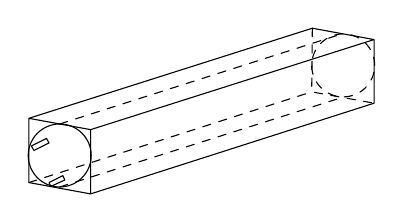
\begin{tikzpicture}[>=stealth,line join=round,line cap=round,font=\footnotesize,scale=0.8]
		\path 
		(0,0) coordinate (O)
		(0.49,0.41) coordinate (A)
		(-0.49,0.59) coordinate (B)
		(-0.49,-0.43) coordinate (C)
		(0.49,-0.61) coordinate (D)
		(4.99,1.84) coordinate (A')
		(4.01,2.02) coordinate (B')
		(4.00,1.01) coordinate (C')
		(4.99,0.83) coordinate (D')
		(4.50,1.43) coordinate (O')
		(0,0.50) coordinate (G)
		(0,-0.50) coordinate (H)
		(4.48,1.93) coordinate (G')
		(4.48,0.92) coordinate (H')
		;
		\draw (O) ellipse (0.5 cm and 0.5 cm);
		\draw[dashed] (O') ellipse (0.5 cm and 0.5 cm);
		\draw (A)--(B)--(C)--(D)--(A)--(A')--(B')--(B) (A')--(D')--(D);
		\draw[dashed] (B')--(C')--(D') (H)--(H') (C)--(C') (G)--(G');
		\draw (-0.45,0.15)--(-0.21,0.27)--(-0.17,0.20)--(-0.41,0.08)--cycle;
		\draw (-0.17,-0.43)--(0.05,-0.32)--(0.08,-0.39)--(-0.14,-0.49)--cycle;
	\end{tikzpicture}
}
\loigiai{
	Vì hộp giấy có chiều dài bằng $0{,}6$ m, đáy là hình vuông cạnh $4$ cm nên bóng đèn huỳnh quanh hình trụ có chiều cao $h=0{,}6$ m $=60$ cm và bán kính đáy $r=\dfrac{4}{2}=2$ cm.\\
	Diện tích xung quanh của bóng đèn là
	$$S_{\text{xq}}=2\pi\cdot r\cdot h=2\pi\cdot2\cdot60=240\pi\ \text{(cm$^2$)}.$$
	Thể tích của bóng đèn là
	$$V=S_{\text{đáy}}\cdot h=\pi r^2\cdot h=\pi\cdot2^2\cdot60=240\pi\ \text{(cm$^3$)}.$$
}
\end{bt}

\begin{bt}%[Dự án EX-9-Đề Cương Toán 9]%[Đặng Thị Lâm]%[9H4V1-4]
Bác An muốn sơn mặt xung quanh của một cây cột có dạng hình trụ với đường kính đáy là $30$ cm và chiều cao là $350$ cm. Chi phí để sơn cây cột đó là $40\,000$ đồng/m$^2$. Hỏi chi phí bác An cần bỏ ra để sơn mặt xung quanh của cây cột đó là bao nhiêu đồng (\textit{lấy $\pi=3{,}14$ và làm tròn kết quả đến hàng nghìn})?
\loigiai{
	Đổi $30$ cm $=0{,}3$ m; $350$ cm $=3{,}5$ m.\\
	Diện tích xung quanh của cây cột là
	$$S_\text{xq}=2\pi rh=2\cdot3{,}14\cdot\dfrac{0{,}3}{2}\cdot3{,}5=3{,}297\ \text{(m$^2$)}.$$
	Chi phí để sơn cây cột là
	$$40\,000\cdot3{,}297=131\,880\ \text{(đồng)}\approx132\,000\ \text{(đồng)}.$$
}
\end{bt}

\begin{bt}%[Dự án EX-9-Đề Cương Toán 9]%[Đặng Thị Lâm]%[9H4V1-4]
\immini{
	Một doanh nghiệp sản xuất vỏ hộp bằng tôn có dạng hình trụ với hai đáy (Hình vẽ). Hình trụ đó có đường kính đáy khoảng $57$ cm và chiều cao khoảng $89$ cm. Chi phí để sản xuất vỏ hộp đó là $100\,000$ đồng/m$^2$. Hỏi số tiền mà doanh nghiệp cần chi để sản suất $1\,000$ vỏ hộp đó là bao nhiêu đồng (\textit{lấy $\pi=3{,}14$ và làm tròn kết quả đến hàng nghìn})?
}
{\begin{tikzpicture}[scale=.8, font=\footnotesize,>=stealth]%<DTools>
		%Gán số liệu.
		%			\draw[gray!50,xstep = 1, ystep = 1] (0,0) grid (5,8);
		
		\def\a{2};\def\b{0.5};\def\h{6};
		%Gán tọa độ.
		\coordinate (O) at (0,0);
		\coordinate (O') at ($(O)+(90:\h)$);
		\coordinate (A) at ($(O)-(0:\a)$);
		\coordinate (B) at ($(O)+(0:\a)$);
		\coordinate (A') at ($(A)+(90:\h)$);
		\coordinate (B') at ($(B)+(90:\h)$);
		%Vẽ khối trụ.
		\shade[left color=gray, right color=gray!10](B') arc (0:360:\a cm and \b cm);
		\draw (B) arc (0:-180:\a cm and \b cm) (B') arc (0:360:\a cm and \b cm) (A)--(A') (B)--(B');
		\draw[stealth-stealth] (2,7)--++(-4,0) node[above,midway] {$57$ cm};
		\draw[stealth-stealth] (3,6)--++(0,-6) node[right,midway] {$89$ cm};
		%\draw[dashed] (B) arc (0:180:\a cm and \b cm);
\end{tikzpicture}}
\loigiai{
	Đổi $57$ cm $=0{,}57$ m; $89$ cm $=0{,}89$ m.\\
	Diện tích toàn phần của hình trụ là
	$$
	S_\text{tp}=2\pi rh+2\pi r^2=\pi dh+2\pi\dfrac{d^2}{4} = 2\cdot 3{,}14\cdot \dfrac{0{,}57}{2}\cdot 0{,}89 + 2\cdot 3{,}14\cdot\left(\dfrac{0{,}57}{2}\right)^2 \approx2{,}103\ (\text{m}^2).$$
	Chi phí để sản xuất một vỏ hộp là
	$$
	100\,000\cdot2{,}103=210\,300\ (\text{đồng}).
	$$
	Chi phí để sản xuất $1\,000$ vỏ hộp là
	$$
	1\,000\cdot210\,300=210\,300\,000\ (\text{đồng}).
	$$
}
\end{bt}

%%==========Bài 18
\begin{bt}%[Dự án EX-9-Đề Cương Toán 9]%[Đặng Thị Lâm]%[9H4V1-4]
	Một đường ống nối hai bể cá trong một thuỷ cung có dạng hình trụ (không có hai đáy), với độ dài (hay chiều cao) là $30$ m và có dung tích là $1\,800\,000~\ell$ (Hình vẽ). Hỏi đường kính đáy của đường ống đó là bao nhiêu mét (lấy $\pi=3{,}14$ và làm tròn kết quả đến hàng phần trăm)?
	\begin{center}
		\begin{tikzpicture}[scale=1, font=\footnotesize,>=stealth,rotate=90]%<DTools>
			%Gán số liệu.
			%			\draw[gray!50,xstep = 1, ystep = 1] (0,0) grid (5,8);
			
			\def\a{2};\def\b{0.5};\def\h{6};
			%Gán tọa độ.
			\coordinate (O) at (0,0);
			\coordinate (O') at ($(O)+(90:\h)$);
			\coordinate (A) at ($(O)-(0:\a)$);
			\coordinate (B) at ($(O)+(0:\a)$);
			\coordinate (A') at ($(A)+(90:\h)$);
			\coordinate (B') at ($(B)+(90:\h)$);
			%Vẽ khối trụ.
			\shade[left color=gray, right color=gray!10](B') arc (0:360:\a cm and \b cm);
			\shade[left color=gray, right color=gray!10](B) arc (0:360:\a cm and \b cm);
			\draw (B) arc (0:-180:\a cm and \b cm) (B') arc (0:360:\a cm and \b cm) (A)--(A') (B)--(B');
			\draw[stealth-stealth] (2,7)--++(-4,0) node[left,midway] {? cm};
			\draw[stealth-stealth] (2.3,6)--++(0,-6) node[above,midway] {30 m};
			\draw[dashed] (B) arc (0:180:\a cm and \b cm);
		\end{tikzpicture}
	\end{center}
	\loigiai{
		Dung tích của đường ống là $1\,800\,000$ lít nên thể tích của đường ống là $1800~\text{m}^3$.\\
		Ta có 
		$$
		V=S_\text{đ}\cdot h = \pi r^2h \text{ suy ra } r = \sqrt{\dfrac{V}{\pi\cdot h}}.
		$$
		Vậy đường kính đáy của đường ống là
		$$
		d= 2r = 2\sqrt{\dfrac{V}{\pi\cdot h}} = 2\sqrt{\dfrac{1\,800}{3{,}14\cdot30}}\approx8{,}74 \,(\text{m}).
		$$
	}
\end{bt}

%%==========Bài 19
\begin{bt}%[Dự án EX-9-Đề Cương Toán 9]%[Đặng Thị Lâm]%[9H4V1-4]
	\immini{
		Pin là nguồn năng lượng phổ biến được sử dụng trong nhiều dụng cụ và thiết bị trong gia đình. Pin $AAA$ (hay pin $3A$) là một loại pin khô, thường được dùng trong những thiết bị điện tử cầm tay, chẳng hạn, điều khiển từ xa ti vi, máy nghe nhạc MP3, \ldots Mỗi chiếc pin $3A$ có dạng hình trụ (hình vẽ), với kích cỡ tiêu chuẩn: chiều cao khoảng $44{,}5$ mm và đường kính đáy khoảng $10{,}5$ mm. Tính diện tích xung quanh, diện tích toàn phần (theo đơn vị centimét vuông) và thể tích (theo đơn vị centimét khối) của một chiếc pin $3A$ đó (\textit{lấy $\pi=3{,}14$ và làm tròn kết quả đến hàng phần mười}).
	}
	{
		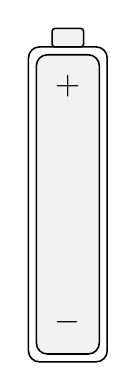
\begin{tikzpicture}[line join = round,line cap = round, >=stealth, thick, font = \small, scale = 1]
			%		\draw[gray!50,xstep = 1, ystep = 1] (0,0) grid (5,5);
			
			\node[rectangle, line width = .2 mm, rounded corners = 4pt, draw = black, anchor = center, outer sep = 0pt, minimum width = 1cm, minimum height = 4cm, rotate = 0] (r1) at (0,2) {};
			\node[rectangle, line width = .2 mm, rounded corners = 4pt, draw = black,fill=gray!10, anchor = center, outer sep = 0pt, minimum width = .8cm, minimum height = 3.8cm, rotate = 0] (r2) at (0,2) {};
			\node[rectangle, line width = .2 mm, rounded corners = 1pt, draw = black,fill=gray!10, anchor = south, outer sep = 0pt, minimum width = .4cm, minimum height = .2cm, rotate = 0] (rr3) at (r1.90) {};
			\path
			(0,3.5) node {\large $+$}
			(0,.5) node {\large $-$}
			;
		\end{tikzpicture}
	}
	\loigiai{
		Đổi đơn vị: $44{,}5$ mm $=4{,}45$ cm; $10{,}5$ mm $= 1{,}05$ cm.\\
		Diện tích xung quanh của chiếc pin là
		$$
		S_\text{xq}=2\pi rh = 2\cdot 3{,}14\cdot\dfrac{1{,}05}{2}\cdot4{,}45\approx14{,}7~(\text{cm}^2).
		$$
		Diện tích toàn phần của chiếc pin là
		$$
		S_\text{tp}=2\pi rh + 2\pi r^2 = 2\cdot 3{,}14\cdot\dfrac{1{,}05}{2} + 2\cdot 3{,}14\cdot\left(\dfrac{1{,}05}{2}\right)^2 \approx 16{,}4\,(\text{cm}^2).
		$$
		Thể tích của chiếc pin là
		$$
		V = \pi r^2h = 3{,}14\cdot\left(\dfrac{1{,}05}{2}\right)^2\cdot4{,}45 \approx3{,}9~(\text{cm}^3).
		$$
	}
\end{bt}

\begin{bt}%[Dự án EX-9-Đề Cương Toán 9]%[Đặng Thị Lâm]%[9H4H1-4]
	Một đoạn ống bằng thép dạng hình trụ có chiều cao $12$ cm, bán kính đáy bên trong $2{,}1$ cm, bán kính đáy bên ngoài $2{,}5$ cm. Người ta muốn sơn toàn bộ mặt bên trong và mặt bên ngoài của đoạn ống này. Tính diện tích cần sơn (kết quả làm tròn đến hàng đơn vị của xăngtimét vuông).
	\loigiai{
		Diện tích xung quanh của mặt bên ngoài ống là
		$$S_1=2\pi r_1h=2\pi\cdot2{,}5\cdot12=60\pi~(\text{cm}^2).$$
		Diện tích xung quanh của mặt bên trong ống là
		$$S_2=2\pi r_2h=2\pi\cdot2{,}1\cdot12=50{,}4\pi~(\text{cm}^2).$$
		Diện tích cần sơn là 
		$$S=S_1+S_2=60\pi+50{,}4\pi=110{,}4\pi\approx347~(\text{cm}^2).$$
	}
\end{bt}

\begin{bt}%[Dự án EX-9-Đề Cương Toán 9]%[Đặng Thị Lâm]%[9H4V1-4]
	\immini{
		Phần bên trong của một máng nước có dạng một nửa hình trụ với đường kính đáy $16$ cm, chiều cao $86$ cm (Hình bên). Tính dung tích của máng nước (\textit{kết quả làm tròn đến hàng đơn vị của lít}).
	}{
		\begin{tikzpicture}[>=stealth,line join=round,line cap=round,font=\footnotesize,scale=1]
			\fill (0,1) circle(1pt);
			\draw (-0.485,1.3)--(0.485,0.7)--(5.985,1.9)--(5.015,2.5)--cycle (0,0.2)--(5.64,1.42);
			\fill (5.5,2.2) circle(1pt);
			\draw (0,0.2) arc [x radius=0.55, y radius=0.8, start angle=270, end angle=157];
			\draw (0,0.2) arc [x radius=0.55, y radius=0.8, start angle=270, end angle=338];
			\draw (5.5,1.4) arc [x radius=0.55, y radius=0.8, start angle=270, end angle=157];
			\draw (5.5,1.4) arc [x radius=0.55, y radius=0.8, start angle=270, end angle=338];
			\fill[color=white] ($(0,0.2)!0.1!(5.64,1.42)$)--(5.64,1.42)--($(5.985,1.9)!0.1!(0.485,0.7)$)--cycle;
			\fill (2.25,1.9) node[above,rotate=11]{$86$ cm};
			\draw[<->] (5.015,2.7)--(6,2.1) node[midway,above,rotate=-34]{$16$ cm};
			%\fill (3,0) node[below]{\textit{Hình 7}};
		\end{tikzpicture}
	}
	\loigiai{
		Bán kính đáy của hình trụ là $\dfrac{16}{2} = 8$ (cm).\\
		Dung tích của máng nước bằng nửa thể tích của hình trụ có cùng bán kính đáy và chiều cao, do đó
		$$V=\dfrac{\pi r^2 h}{2}=\dfrac{\pi\cdot8^2\cdot86}{2}=2\,752\pi\textrm{ (cm$^3$)}\approx9~\text{(l)}.$$
	}
\end{bt}

\begin{bt}%[Dự án EX-9-Đề Cương Toán 9]%[Đặng Thị Lâm]%[9H4H1-4]
	Một bể nước hình trụ có bán kính đáy $r=1{,}2$ m (tính từ tâm bể đến mép ngoài), bề dày của thành bể là $b=0{,}05$ m, chiều cao lòng bể là $h=1{,}6$ m. Tính dung tích của bể nước (kết quả làm tròn đến hàng phần nghìn).
	\begin{center}
		\begin{tikzpicture}[>=stealth,line join=round,line cap=round,font=\footnotesize,scale=1]
			\def\a{1.5};\def\b{0.3};\def\c{3};
			\fill[cyan!20] ($(1.8,0)+(90:\c)$) arc(0:360:1.8 cm and 0.5 cm);
			\fill[white] (90:\c) ellipse (\a cm and \b cm);
			\draw[dashed] (0,0) ellipse (\a cm and \b cm)
			(1.8,0) arc(0:180:1.8 cm and 0.5 cm)
			(\a,0)--++(90:\c) (-\a,0)--++(90:\c)
			(0,0)--++(90:\c)node[midway,right]{\scriptsize $h$}--++(0:1.8)node[midway,sloped,fill=white]{\scriptsize $R$};
			\draw (-1.8,0) arc(180:360:1.8 cm and 0.5 cm)
			(90:\c) ellipse (\a cm and \b cm)
			($(1.8,0)+(90:\c)$) arc(0:360:1.8 cm and 0.5 cm)
			(1.8,0)--++(90:\c) (-1.8,0)--++(90:\c);
			\draw[dashed] (-1.5,\c)--++(180:0.3)node[pos=0.2,above=-0.1cm]{\scriptsize $b$};
			\foreach \y in {0,\c}{\fill (0,\y) circle (1.5pt);}
		\end{tikzpicture}
	\end{center}
	\loigiai{
		Dung tích của bể nước là $V=S_{\textrm{đáy}}h=\pi(1{,}2-0{,}05)^2\cdot1{,}6 = \dfrac{529\pi}{250} \approx6{,}648\ (\text{m}^3)$.
	}
\end{bt}

\begin{bt}%[Dự án EX-9-Đề Cương Toán 9]%[Đặng Thị Lâm]%[9H4V1-4]
	Một ống kim loại dạng hình trụ có chiều dài $35$ cm, đường kính đáy bên trong và bên ngoài của ống lần lượt là $20$\,mm và $28$\,mm (Hình bên). Tính thể tích của phần kim loại sử dụng để làm ống (\textit{kết quả làm tròn đến hàng đơn vị centimét khối}).
	\begin{center}
		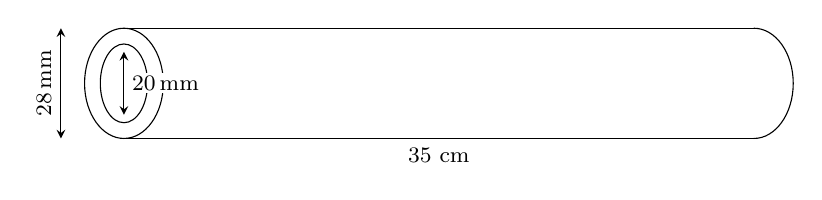
\begin{tikzpicture}[>=stealth,line join=round,line cap=round,font=\footnotesize,scale=1]
			\draw (0,0)--(8,0) (0,1.4)--(8,1.4);
			\draw (0,0.7) ellipse (0.5 cm and 0.7 cm);
			\draw (0,0.7) ellipse (0.3 cm and 0.5 cm);
			\draw (8,0) arc [x radius=0.5, y radius=0.7, start angle=-90, end angle=90];
			\draw[<->] (-0.8,0)--(-0.8,1.4) node[midway,above,rotate=90]{$28$\,mm};
			\draw[<->] (0,0.3)--(0,1.1) node[midway,right,fill=white, inner sep = 1pt, outer sep = 2pt]{$20$\,mm};
			\fill (4,0) node[below]{$35$ cm};
			%\fill (4,-0.5) node[below]{\textit{Hình 8}};
		\end{tikzpicture}
	\end{center}
	\loigiai{
		Đổi đơn vị: $20$ mm $= 2$ cm; $28$ mm $= 2{,}8$ cm.\\
		Thể tích của khối kim loại bằng hiệu thể tích hình trụ bên ngoài và thể tích hình trụ bên trong của khối, do đó
		$$V=\pi\cdot\left(\dfrac{2{,}8}{2}\right)^2\cdot35 - \pi\cdot\left(\dfrac{2}{2}\right)^2\cdot35\approx 106~(\text{cm}^3).$$
	}
\end{bt}

\begin{bt}%[Dự án EX-9-Đề Cương Toán 9]%[Đặng Thị Lâm]%[9H4V1-4]
	\immini{
		Từ một hình trụ có đường kính đáy $24$ cm và chiều cao $32$ cm, người ta khoét bỏ một hình trụ có đường kính đáy $10$ cm và chiều cao $14$ cm (Hình bên).
		\begin{enumerate}
			\item Tính thể tích của phần còn lại của hình trụ.
			\item Người ta sơn toàn bộ các mặt của phần còn lại của hình trụ. Tính diện tích được phủ sơn (\textit{kết quả làm tròn đến hàng đơn vị của centimét vuông}).
		\end{enumerate}
	}{
		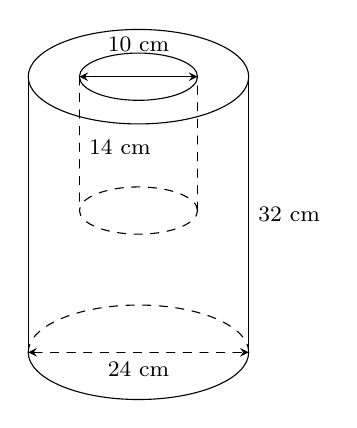
\begin{tikzpicture}[>=stealth,line join=round,line cap=round,font=\footnotesize,scale=1]
			\draw (0,0)--(0,3.5) (2.8,0)--(2.8,3.5);
			\draw (1.4,3.5) ellipse (1.4 cm and 0.6 cm);
			\draw (0,0) arc [x radius=1.4, y radius=0.6, start angle=180, end angle=360];
			\draw[dashed] (2.8,0) arc [x radius=1.4, y radius=0.6, start angle=0, end angle=180];
			\draw[dashed,<->] (0,0)--(2.8,0) node[midway,below]{$24$ cm};
			\fill (2.8,1.75) node[right]{$32$ cm};
			\draw (1.4,3.5) ellipse (0.75 cm and 0.3 cm);
			\draw[<->] (0.65,3.5)--(2.15,3.5);
			\fill (1.4,3.7) node[above]{$10$ cm};
			\draw[dashed] (0.65,3.5)--(0.65,1.8) (2.15,1.8)--(2.15,3.5);
			\draw[dashed] (1.4,1.8) ellipse (0.75 cm and 0.3 cm);
			\fill (0.65,2.6) node[right]{$14$ cm};
			%\fill (1.4,-0.8) node[below]{\textit{Hình 9}};
		\end{tikzpicture}
	}
	\loigiai{
		\begin{enumerate}
			\item Thể tích của hình trụ ban đầu là $V_1=\pi\cdot12^2\cdot32=4\,608\pi$ (cm$^3$).\\
			Thể tích của hình trụ được lấy ra là $V_2=\pi\cdot5^2\cdot14=350\pi$ (cm$^3$).\\
			Thể tích của phần gỗ còn lại là $V=V_1-V_2=4\,608\pi-350\pi=4\,258\pi$ (cm$^3$).
			\item Diện tích toàn phần của hình trụ ban đầu là
			$$S_1=2\pi\cdot12\cdot32+2\pi\cdot12^2=1\,056\pi\textrm{ (cm$^2$)}.$$
			Diện tích xung quanh của hình trụ lấy đi là $S_2=2\pi\cdot5\cdot14=140\pi$ (cm$^2$).\\
			Diện tích cần sơn là $S=S_1+S_2=1\,056\pi+140\pi=1\,196\pi\approx3\,757$ (cm$^2$).
		\end{enumerate}
	}
\end{bt}

\begin{bt}%[Dự án EX-9-Đề Cương Toán 9]%[Đặng Thị Lâm]%[9H4V1-4]
	\immini{Một vật thể rắn hình chữ $C$ dạng nửa hình trụ có bán kính bên trong là $8$ cm và độ dày đồng đều là $1{,}6$ cm có chiều cao là $10$ cm (Hình 3). Tìm thể tích của vật thể (kết quả làm tròn đến hàng đơn vị của centimét khối).}
	{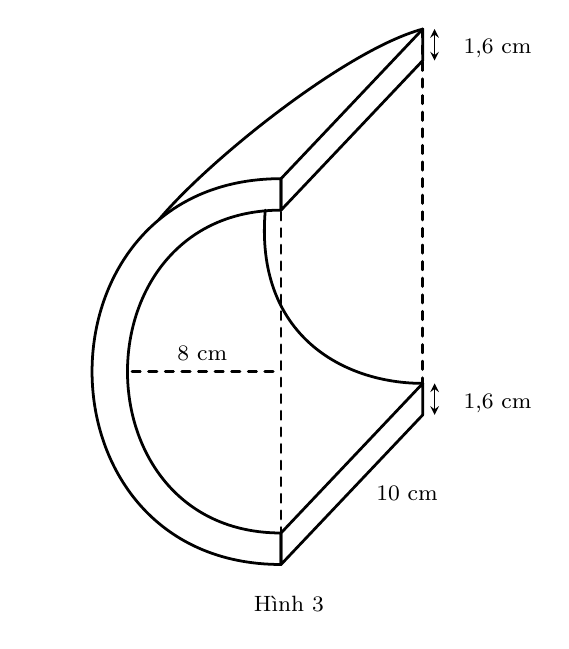
\begin{tikzpicture}[line join=round, line cap=round,>=stealth,font=\footnotesize,scale=1]    
			\draw[line width=1pt] 
			(2.4,0)..controls +(180:3.2) and +(180:3.2)..(2.4,4.9)--++(0,-0.4)
			..controls +(180:2.6) and +(180:2.6)..++(0,-4.1)--cycle
			;
			\draw[line width=1pt] (0.85,4.38) ..controls +(50:1) and +(-165:1).. (2.4+1.8,4.9+1.9);
			\draw[line width=1pt] (4.2,2.3)..controls +(180:1) and +(-95:1.6).. (2.2,4.5); 
			\draw[line width=1pt] (2.4,4.9)--++(1.8,1.9)--++(0,-0.4)--++(-1.8,-1.9)--cycle;
			\draw[line width=1pt,yshift=-4.5cm] (2.4,4.9)--++(1.8,1.9)--++(0,-0.4)--++(-1.8,-1.9)--cycle;
			\draw[dashed,line width=1pt] (2.4,4.9)--++(0,-0.4) --++(0,-4.1);
			\draw[dashed,line width=1pt,yshift=1.9cm,xshift=1.8cm] (2.4,4.9)--++(0,-0.4) --++(0,-4.1);
			\draw[dashed,line width=1pt] (2.3,2.45)--(0.5,2.45)node[above,pos=0.5]{$8$ cm};
			\draw (4,0.9)node[]{$10$ cm}(5.15,2.05)node[]{$1{,}6$ cm}(5.15,6.55)node[]{$1{,}6$ cm};
			\draw[<->] (4.35,1.9)--(4.35,2.3);\draw[<->] (4.35,1.9+4.5)--(4.35,2.3+4.5);
			\draw (2.5,-0.5)node{Hình 3};        
	\end{tikzpicture}}
	\loigiai{
		Thể tích của vật thể là $V=\dfrac{1}{2}\left[\pi\cdot(8+1{,}6)^2\cdot10-\pi\cdot8^2\cdot10\right]\approx442~(\text{cm}^3)$.    
	}
\end{bt}

\begin{bt}%[Dự án EX-9-Đề Cương Toán 9]%[Đặng Thị Lâm]%[9H4V1-4]
	\immini{Một khối thuỷ tinh được tạo thành từ một phần dạng hình hộp chữ nhật có kích thước $6$ cm, $16$ cm, $9$ cm và một phần dạng nửa hình trụ có đường kính đáy $6$ cm, chiều cao $16$ cm (Hình bên). Tính
		\begin{enumerate}
			\item Thể tích của khối thuỷ tinh.
			\item Diện tích bề mặt của khối thuỷ tinh.
			(\textit{Làm tròn kết quả đến hàng đơn vị của xăng ti mét khối, centimét vuông}).
	\end{enumerate}}
	{\begin{tikzpicture}[>=stealth,line join=round,line cap=round]
			\draw[dashed,black,scale=2.5] (0,0)coordinate(A)--(-150:2.0)coordinate(B) (1,0)coordinate(D)--(A)--($(A)+(90:1.3)$)coordinate(A');
			\draw[black,scale=2.5] (B)--($(D)-(A)+(B)$)coordinate(C)--(D)--($(D)+(90:1.3)$)coordinate(D')($(B)+(90:1.3)$)coordinate(B')--($(D')-(A')+(B')$)coordinate(C')--(D') (C')--(C) (B')--(B);
			\draw[black] (C') arc (0:180:1.25cm);
			\draw[black] (D') arc (0:120:1.25cm);
			\draw[black,dashed] (D') arc (0:180:1.25cm);
			\draw [dashed] (B')--(A')--(D');
			\coordinate (I) at ($(B')!0.5!(C')$);
			\coordinate (I') at ($(A')!0.5!(D')$);
			\coordinate (T) at ($(I)!1!-60:(B')$);
			\coordinate (T') at ($(I')!1!-60:(A')$);
			\draw (T)--(T');
			\path (B')--(B)node[pos=0.5,sloped,black,below left]{$9$ cm};
			\path (C)--(B)node[pos=0.5,sloped,black,below]{$6$ cm};
			\path (C)--(D)node[pos=0.5,sloped,black,below right]{$16$ cm};
			%\draw (.5,-2.5)node{Hình 1};
	\end{tikzpicture}}
	\loigiai{
		\begin{enumerate}
			\item Thể tích của phần dạng hình hộp chữ nhật là $V_1=16\cdot6\cdot9=864$ (cm$^3$).\\    
			Thể tích của phần dạng nửa hình trụ là $V_2=\dfrac{\pi\cdot3^2\cdot16}{2}=72\pi$ (cm$^3$).\\     
			Thể tích của khối thuỷ tinh là $V=V_1+V_2=864+72\pi\approx1090$ (cm$^3$).\\    
			\item Diện tích bề mặt phần có dạng hình hộp chữ nhật của khối thuỷ tinh là
			$$S_1=6\cdot16+2(9\cdot16+6\cdot9)=492~(\text{cm}^2).$$    
			Diện tích bề mặt phần có dạng nửa hình trụ của khối thuỷ tinh là
			$$S_2=\dfrac{2\cdot\pi\cdot3\cdot16+2\cdot\pi\cdot3^2}{2}=57\pi~(\text{cm}^2).$$    
			Tổng diện tích bề mặt của khối thuỷ tinh là $S=S_1+S_2=492+57\pi\approx671~(\text{cm}^2)$.
		\end{enumerate}    
	}
\end{bt}

\begin{bt}%[Dự án EX-9-Đề Cương Toán 9]%[Đặng Thị Lâm]%[9H4V1-4]
	\immini{Một khối hộp chữ nhật đặc với kích thước ba cạnh là $12$ cm, $10$ cm, $7$ cm bị khoét bởi một nửa hình trụ có đường kính $4$ cm và chiều dài $12$ cm (Hình bên). Tính
		\begin{enumerate}
			\item Thể tích của khối còn lại.
			\item Diện tích bề mặt của khối còn lại.
			(\textit{Làm tròn kết quả đến hàng đơn vị của centimét khối, centimét vuông}).
		\end{enumerate}
	}{
		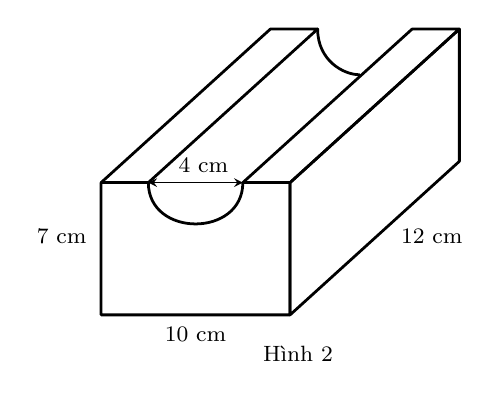
\begin{tikzpicture}[line join = round, line cap=round,>=stealth,font=\footnotesize,scale=1]
			
			\draw[line width=1pt] (0,0)--(0,1.68)--++(0.6,0)
			..controls +(-90:0.7) and +(-90:0.7)..++(1.2,0)
			--++(0.6,0)--++(0,-1.68)--cycle;
			\draw[line width=1pt] (0,1.68)--++(2.15,1.95)--++(0.6,0)--++(-2.15,-1.95)--cycle;
			\draw[line width=1pt,xshift=1.8cm] (0,1.68)--++(2.15,1.95)--++(0.6,0)--++(-2.15,-1.95)--cycle;
			\draw[line width=1pt] (2.4,0)--(2.4,1.68)--++(2.15,1.95)--++(0,-1.68)--cycle;
			\draw[line width=1pt] (2.75,3.63)..controls +(-90:0.4) and +(180:0.2) ..(3.28,3.05);
			\draw (1.2,-0.25) node{$10$ cm}(1.3,1.9) node{$4$ cm}
			(4.2,1) node{$12$ cm}(-0.5,1) node{$7$ cm}
			(2.5,-0.5) node[]{Hình 2}
			;
			\draw[<->] (0.6,1.68)--(1.8,1.68);
	\end{tikzpicture}}
	\loigiai{
		\begin{enumerate}
			\item Thể tích của khối hộp chữ nhật khi chưa bị khoét là
			$$
			V_1=12\cdot10\cdot7=840~(\text{cm}^3).
			$$    
			Thể tích của nửa hình trụ là $V_2=\dfrac{1}{2}\pi r^2h=\dfrac{1}{2}\cdot\pi\cdot2^2\cdot12=24\pi~(\text{cm}^3).$\\
			Thể tích của khối còn lại là $V=V_1-V_2=840-24\pi\approx765~(\text{cm}^3).$
			\item Diện tích toàn phần của khối hộp khi chưa bị khoét là
			$$S_1=2(7\cdot10+12\cdot10+7\cdot12)=548~(\text{cm}^2).$$
			Diện tích xung quanh của nửa hình trụ là $S_2=\pi rh=\pi\cdot2\cdot12=24\pi~(\text{cm}^2).$\\
			Diện tích hai đáy của nửa hình trụ là $S_3=\pi r^2=4\pi~(\text{cm}^2).$\\
			Diện tích mặt cắt dọc của nửa hình trụ là $S_4=4\cdot12=48~(\text{cm}^2).$\\
			Diện tích bề mặt của khối còn lại là
			$$S=S_1+S_2-S_3-S_4=548+24\pi-4\pi-48\approx599~(\text{cm}^2).$$
		\end{enumerate}    
	}
\end{bt}

\begin{bt}%[Dự án EX-9-Đề Cương Toán 9]%[Đặng Thị Lâm]%[9H4V1-4]
	\immini{
		Một thùng đựng nước có dạng hình trụ với chiều cao là $35$ cm và đường kính đáy là $30$ cm.
		\begin{enumerate}
			\item Tính thể tích của thùng nước. (\textit{kết quả làm tròn đến hàng đơn vị}).
			\item Người ta sử dụng thùng nước trên để múc nước đổ vào một bể chứa có dung tích $1$ m$^3$. Hỏi cần phải đổ ít nhất bao nhiêu thùng nước thì đầy bể chứa? Biết rằng, mỗi lần xách người ta chỉ đổ đầy $90\%$ thùng để nước không đổ ra ngoài. Cho công thức tính thể tích hình trụ: $V=\pi r^2\cdot h$ trong đó $h$ là chiều cao hình trụ, $r$ là bán kính đường tròn đáy.
		\end{enumerate}
	}{
		\begin{tikzpicture}[>=stealth,line join=round,line cap=round,font=\footnotesize,scale=1]
			\def\x{1.4}
			\def\y{0.6}
			\coordinate (O) at (0,0);
			\coordinate (O') at ($(O)+(0,3.1)$);
			\coordinate (N) at ($(O)+(0,3)$);
			\path[fill=cyan!40] (N) arc (0:180:\x cm and \y cm)--($(O)+(-2*\x,0)$) arc (180:360:\x cm and \y cm) --cycle;
			\draw[dashed,blue] (N) arc (0:180:\x cm and \y cm);
			%\node[circle,outer color=white!80!black,inner color=white,minimum width=1.2cm] (radial) at (-5.7,2.5) {};
			\draw[dashed,blue] (N) arc (0:-180:\x cm and \y cm);
			%\draw[dashed] (O) arc (0:180:\x cm and \y cm);
			\draw (O) arc (0:-180:\x cm and \y cm);
			
			\draw (O)--(O') ($(O)+(-2*\x,0)$)--($(O')+(-2*\x,0)$);
			
			\fill (N) circle(2pt) node{$N$};
			\path[fill=cyan!40] (0.3,3.1) arc (0:180:1.7 cm and 0.6 cm)--(-3.1,2.6) arc (180:360:1.7 cm and 0.6 cm) --cycle;
			\draw (0.3,3.1) arc (0:180:1.7 cm and 0.6 cm)--(-3.1,2.6) arc (180:360:1.7 cm and 0.6 cm) --cycle;
			\draw (-3.1,3.1) arc (180:360:1.7 cm and 0.6 cm);
			\draw (O') arc (0:360:\x cm and 0.45 cm);
			\fill[cyan!10] (O') arc (0:360:\x cm and 0.45 cm);
		\end{tikzpicture}
	}
	\loigiai{
		\begin{enumerate}
			\item Thể tích của thùng nước là
			$$V=\pi\cdot\left(\dfrac{30}{2}\right)^2\cdot35=7\,875\pi\approx24\,740~(\text{cm}^3).$$
			\item Đổi $1$ m$^3=1\,000\,000$ cm$^3$.\\
			Số thùng nước ít nhất cần phải đổ để đầy bể chứa là
			$$1\,000\,000:(7\,875\pi\cdot90\%)\approx45\text{ (thùng)}.$$
			Vậy cần phải đổ ít nhất $45$ thùng nước thì đầy bể chứa.
		\end{enumerate}
	}
\end{bt} 

\begin{bt}%[Dự án EX-9-Đề Cương Toán 9]%[Đặng Thị Lâm]%[9H4V1-4]
	Một bồn hình trụ đang chứa dầu, được đặt nằm ngang, có chiều dài bồn là $5$ m, bán kính đáy $1$ m, với nắp bồn đặt trên mặt nằm ngang của hình trụ. Người ta đã rút dầu trong bồn tương ứng với $0{,}5$ m của đường kính đáy (như hình vẽ). Tính lượng dầu còn lại trong bồn (giả sử độ dày của bồn là không đáng kể và kết quả làm tròn đến chữ số thập phân thứ $2$). \\
	Biết $V_{\text{hình trụ}}=\pi R^2h$ trong đó $R$ là bán kính đáy, $h$ là chiều cao hình trụ và \\
	Thể tích dầu rút ra$=$Diện tích mặt đáy phần dầu rút ra$\times$Chiều cao hình trụ.
	\begin{center}
		\begin{tikzpicture}[declare function={r1=1.5;r2=2;},line join=round,line cap=round,font=\footnotesize,scale=1,>=stealth]
			\path 
			(40:r1 and r2) coordinate (A)
			($(A)+(8,0)$) coordinate (B)
			(160:r1 and r2) coordinate (C)
			($(C)+(8,0)$) coordinate (D)
			;
			\fill[gray!25] 
			(A)--(B) arc (40:-90:r1 and r2)--(-90:r1 and r2)
			arc (270:160: r1 and r2)--(C)
			;
			\draw[dashed]
			(90:r1 and r2) arc (90:-90: r1 and r2)
			(C)--(A)--(B)
			;
			\draw 
			(B)--(D)--(C)
			(270:r1 and r2) arc (270:90:r1 and r2) 
			%(0,0) ellipse (r1 and r2)
			(8,0) ellipse (r1 and r2)
			(90:r2)--($(90:r2)+(8,0)$)
			(-90:r2)--($(-90:r2)+(8,0)$)
			;
			\path 
			(8,0) coordinate (O)
			($(90:r2)+(O)$) coordinate (E)
			(intersection of D--B and O--E) coordinate (M)
			;
			\draw 
			(E)--(M) node[midway,right=-2pt] {$0{,}5$ m}
			;
			\fill
			(O) circle (1pt)
			;
			\draw [dashed] (O)--($(O)+(r1,0)$) node[midway, below] {$1$ m}
			%ghi chú
			(-90:r2)--($(-90:r2)+(0,-0.5)$)
			($(-90:r2)+(O)$)--($(-90:r2)+(O)+(0,-0.5)$)
			;
			\draw[<->] 
			($(-90:r2)+(0,-0.5)$)--($(-90:r2)+(O)+(0,-0.5)$) node[midway,above] {$5$ m}
			;
		\end{tikzpicture}
		%--------------------------------------------------------------	
		\quad
		\begin{tikzpicture}[declare function={r=2.2;},line join=round,line cap=round,font=\footnotesize,scale=1]
			\path (0,0) coordinate (O)
			(30:r) coordinate (C)
			(150:r) coordinate (A)
			(90:r) coordinate (B)
			($(A)!0.5!(C)$) coordinate (H)
			;
			\fill[blue!25] 
			(C) arc (30:150:r)--(C)
			;
			\draw 
			(O) circle (r)
			(O)--(A)--(C)--cycle
			(H)--(B)
			;
			\draw [dashed]
			(O)--(H)
			;
			\foreach \t/\g in {A/120,B/90,C/60,H/-50,O/-90}{
				\path (\t) node[shift={(\g:7pt)}]{$\t$};
			}
		\end{tikzpicture}
	\end{center}
	\loigiai{
		Ta có $OH=OB-BH=1-0{,}5=0{,}5$ (m).\\
		Xét $\triangle OHC$ vuông tại $H$, ta có
		$$\cos\widehat{HOC}=\dfrac{OH}{OC}=\dfrac{0{,}5}{1}=0{,}5.$$
		Suy ra $\widehat{HOC}=60^\circ$ và $\widehat{AOC}=2\cdot60^\circ=120^\circ$.\\
		Ta có $AC=2HC=2OC\cdot\sin\widehat{HOC}=2\cdot1\cdot\dfrac{\sqrt{3}}{2}=\sqrt{3}$ (m).\\
		Diện tích mặt đáy phần dầu rút ra
		$$S_{\text{quạt}AOC}-S_{\triangle AOC}
		=\dfrac{\pi\cdot1^2\cdot120}{360}-\dfrac{1}{2}\cdot0{,}5\cdot\sqrt{3}
		=\dfrac{\pi}{3}-\dfrac{\sqrt{3}}{4}~(\text{m}^2).$$
		Thể tích dầu rút ra
		$$5\left(\dfrac{\pi}{3}-\dfrac{\sqrt{3}}{4}\right)~(\text{m}^3).$$
		Thể tích hình trụ
		$$V_{\text{hình trụ}}=\pi R^2h=\pi\cdot1^2\cdot5=5\pi~(\text{m}^3).$$
		Lượng dầu còn lại trong bồn
		$$5\pi-5\left(\dfrac{\pi}{3}-\dfrac{\sqrt{3}}{4}\right)\approx12{,}64~(\text{m}^3).$$
	}
\end{bt}

\begin{bt}%[Dự án EX-9-Đề Cương Toán 9]%[Đặng Thị Lâm]%[9H4V1-4]
	\immini{
		Gạch chống nóng $6$ lỗ còn được gọi là gạch Tuynel, có dạng hình hộp chữ nhật với kích thước $195$ mm$\times135$ mm$\times90$ mm. Mỗi viên gạch có $6$ lỗ rỗng hình trụ bằng nhau phía bên trong, mỗi lỗ rỗng này có đường kính đáy $28$ mm. 
		\begin{enumerate}
			\item Tính thể tích nguyên vật liệu để làm nên một viên gạch trên (bỏ qua phần viền của viên gạch). Biết thể tích hình trụ là $V=\pi R^2h$, trong đó $R$ là bán kính đáy, $h$ là chiều cao hình trụ, lấy $\pi=3{,}14$.
			\item Một xe tải dùng để chở gạch có thùng xe là một hình hộp chữ nhật với kích thước $2{,}1$ m$\times1{,}5$ m$\times1{,}5$ m. Mỗi chuyến xe chở gạch chỉ chở được tối đa $90\%$ sức chứa thùng xe. Một công trình cần xây dựng $180$ m$^2$ tường và khi thi công, người ta mua dư thêm $2\%$ để phòng hư hao. Hỏi cần chở ít nhất bao nhiêu chuyến để đáp ứng nhu cầu xây dựng như trên. Biết rằng cứ $1$ m$^2$ tường nhà thì cần $55$ viên gạch.
		\end{enumerate}
	}{
		\begin{tikzpicture}[font=\footnotesize,line join=round, line cap=round, >=stealth]
			\path
			(1,0) coordinate (C)
			(0,0.58) coordinate (D)
			($(D)+(90:2)$) coordinate (E)
			($(E)!.5!(C)$) coordinate (F1)
			($(D)!2!(F1)$) coordinate (F)
			($(C)+(30:2.5)$) coordinate (I)
			($(F)+(I)-(C)$) coordinate (H)
			($(E)+(I)-(C)$) coordinate (G)
			($(D)!1/4!(E)$) coordinate (D1)
			($(C)!1/4!(F)$) coordinate (C1)
			($(D)!1/2!(E)$) coordinate (D2)
			($(C)!1/2!(F)$) coordinate (C2)
			($(D)!3/4!(E)$) coordinate (D3)
			($(C)!3/4!(F)$) coordinate (C3)
			;
			\draw (C)--(D)--(E)--(F)--cycle (C)--(I) (F)--(H) (E)--(G)--(H)--(I);
			\draw[rotate=45] ($(D1)!1/4!(C1)$) ellipse (1ex and 1.3ex);
			\draw[rotate=45] ($(D1)!3/4!(C1)$) ellipse (1ex and 1.3ex);
			\draw[rotate=45] ($(D2)!1/4!(C2)$) ellipse (1ex and 1.3ex);
			\draw[rotate=45] ($(D2)!3/4!(C2)$) ellipse (1ex and 1.3ex);
			\draw[rotate=45] ($(D3)!1/4!(C3)$) ellipse (1ex and 1.3ex);
			\draw[rotate=45] ($(D3)!3/4!(C3)$) ellipse (1ex and 1.3ex);
			\draw[<->] ($(D)+(-120:1.5ex)$)--($(C)+(-120:1.5ex)$)node[midway,rotate=-30,below]{$90$ mm};
			\draw[<->] ($(C)+(-45:1.5ex)$)--($(I)+(-45:1.5ex)$)node[midway,rotate=30,below]{$195$ mm};
			\draw[<->] ($(H)+(0:1.5ex)$)--($(I)+(0:1.5ex)$)node[midway,rotate=-90,above]{$135$ mm};
			%\foreach \i/\j in{C/90,D/90,E/90,F/90,I/90} \fill[black] (\i) circle (1.5pt) node[shift=(\j:2.5mm)] {$ \i $};
		\end{tikzpicture}
	}
	\loigiai
	{
		\begin{enumerate}
			\item Thể tích $6$ lỗ hình trụ là $6\pi R^2h=6\cdot3{,}14\cdot(28:2)^2\cdot195=720\,064{,}8$ (mm$^3$).\\
			Thể tích viên gạch là $195\cdot135\cdot90=2\,369\,250$ (mm$^3$).\\
			Thể tích nguyên vật liệu để làm nên một viên gạch là $2\,369\,250-720\,064{,}8=1\,649\,185{,}2$ (mm$^3$).
			\item Số viên gạch cần là $180\cdot55\cdot(1+2\%)=10\,098$ (viên).\\
			Thể tích $1$ viên gạch là $2\,369\,250$ (mm$^3$) $=0{,}00236925$ (m$^3$).\\
			Số viên gạch chở được mỗi chuyến là $(2{,1}\cdot1{,}5\cdot1{,}5)\cdot90\%:0{,}00236925=\dfrac{70\,000}{39}$ (viên).\\
			Số chuyến ít nhất cần chở là $10\,098:\dfrac{70\,000}{39}\approx6$ (xe).\\
			Vậy cần chở ít nhất $6$ chuyến xe để đáp ứng nhu cầu xây dựng như trên.
		\end{enumerate}
	}
\end{bt} 

\begin{bt}%[Dự án EX-9-Đề Cương Toán 9]%[Đặng Thị Lâm]%[9H4V1-4]
	Để tổ chức sinh nhật cho con gái, chị Thanh đã đặt thợ làm bánh tại cửa hàng Bakery với yêu cầu bánh được làm hai tầng, mỗi tầng cao $15$ cm, bán kính tầng trên là $15$ cm, đường kính tầng dưới là $40$ cm.
	Biết công thức tính thể tích khối trụ là $V=\pi r^2h$ và diện tích xung quanh hình trụ là $S_{xq}=2\pi rh$ với $r$ là bán kính, $h$ là chiều cao.
	\begin{center}
		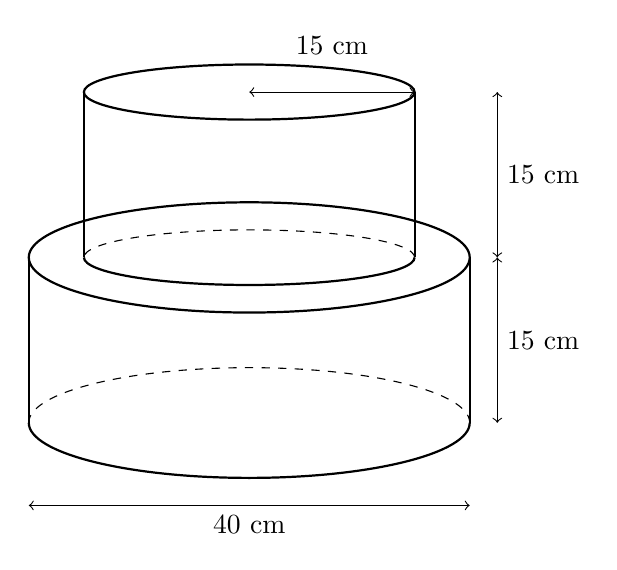
\begin{tikzpicture}[scale=0.7]
			% Khối trụ lớn
			\draw[thick] (0,0) ellipse (4cm and 1cm);
			\draw[thick] (-4,0) -- (-4,-3);
			\draw[thick] (4,0) -- (4,-3);
			\draw[thick] (-4,-3) arc (180:360:4cm and 1cm);
			\draw[dashed] (4,-3) arc (0:180:4cm and 1cm);
			% Khối trụ nhỏ
			\draw[thick] (0,3) ellipse (3cm and 0.5cm);
			\draw[thick] (-3,3) -- (-3,0);
			\draw[thick] (3,3) -- (3,0);
			\draw[thick] (-3,0) arc (180:360:3cm and 0.5cm);
			\draw[dashed] (3,0) arc (0:180:3cm and 0.5cm);
			% Kích thước
			\draw[<->] (-4,-4.5) -- (4,-4.5) node[midway, below] {$40$ cm};
			\draw[<->] (4.5,-3) -- (4.5,0) node[midway, right] {$15$ cm};
			\draw[<->] (4.5,0) -- (4.5,3) node[midway, right] {$15$ cm};
			\draw[<->] (0,3) -- (3,3);
			\fill (1.5,3.5) node[above] {$15$ cm};
		\end{tikzpicture}
	\end{center}
	\begin{enumerate}
		\item Tính thể tích chiếc bánh. (\textit{Làm tròn kết quả đến hai chữ số thập phân})
		\item Hỏi với kích thước yêu cầu của chị Thanh, khi chiếc bánh được hoàn thành thì người thợ có tất cả bao nhiêu diện tích bề mặt để trang trí bánh? (\textit{Làm tròn kết quả đến hai chữ số thập phân}).
	\end{enumerate}
	\loigiai
	{
		\begin{enumerate}
			\item Thể tích tầng trên chiếc bánh là $V_1=\pi r_1^2h_1=\pi\cdot15^2\cdot15=3\,375\pi$ (cm$^3$).\\
			Bán kính của tầng dưới của chiếc bánh là $r_2=\dfrac{40}{2}=20$ (cm).\\
			Thể tích tầng dưới chiếc bánh là $V_2=\pi r_2^2h_2=\pi\cdot20^2\cdot15=6\,000\pi$ (cm$^3$).\\
			Thể tích toàn bộ chiếc bánh là 
			$V=V_1+V_2=3\,375\pi+6\,000\pi=9\,375\pi\approx29\,452{,}43$ (cm$^3$).
			\item 
			Diện tích xung quanh tầng trên là
			$S_{xq1}=2\pi r_1h_1=2\pi\cdot15\cdot15=450\pi$ (cm$^2$).\\
			Diện tích xung quanh tầng dưới là
			$S_{xq2}=2\pi r_2h_2=2\pi\cdot20\cdot15=600\pi$ (cm$^2$).\\
			Diện tích mặt trên tầng trên là
			$S_{mt1}=\pi r_1^2=\pi\cdot15^2=225\pi$ (cm$^2$).\\
			Diện tích mặt trên tầng dưới (không tính phần chồng với tầng trên) là
			$$S_{mt2}=\pi r_2^2-\pi r_1^2=\pi\cdot20^2-\pi\cdot15^2=175\pi~(\text{cm}^2).$$
			Tổng diện tích bề mặt để trang trí là
			$$S=S_{xq1}+S_{xq2}+S_{mt1}+S_{mt2}=450\pi+600\pi+225\pi+175\pi=1\,450\pi\approx4\,555{,}31~(\text{cm}^2).$$
		\end{enumerate}
	}
\end{bt} 

\begin{bt}%[Dự án EX-9-Đề Cương Toán 9]%[Đặng Thị Lâm]%[9H4V1-4]
	\immini{
		Trong hình vẽ, $6$ lon nước ngọt hình trụ được đặt sát nhau trong thùng carton có dạng hình hộp chữ nhật. Mỗi lon có đường kính $7$ cm và chiều cao $11$ cm.
		\begin{enumerate}
			\item Tính thể tích thùng carton.
			\item Tính tỉ số phần trăm ($\%$) giữa thể tích phần còn trống trong thùng carton khi đựng $6$lon nước ngọt với thể tích của thùng carton (\textit{kết quả làm tròn đến hàng phần mười}). Biết thể tích hình trụ là $V=\pi\cdot R^2\cdot h$ trong đó $R$ là bán kính đáy; $h$ là chiều cao hình trụ.
		\end{enumerate}
	}{
		\begin{tikzpicture}[line join=round, line cap=round,>=stealth,font=\footnotesize,scale=.45,transform shape]
			\tikzset{tru/.pic={ 
					\def\a{2}
					\draw[fill=cyan!10] (0,0) arc(180:360:2cm and 0.75cm)--(\a*2,5) arc(0:180:2cm and 0.75cm)--cycle;
					\draw  (\a*2,5) arc(0:-180:2cm and 0.75cm);  
			}}
			\path
			(0,5)coordinate (A)--(0.5,6.5) coordinate (B)
			(12,5)coordinate (D)--(12.5,6.5)coordinate (C)
			(2,4.25)coordinate (E)--(10,4.25)coordinate (F)
			(2+0.5,7.25)coordinate (H)--(10+0.5,7.25)coordinate (G)
			(intersection of A--B and H--G) coordinate (R) 
			(intersection of C--D and H--G) coordinate (Q) 
			(intersection of C--D and E--F) coordinate (T)
			(intersection of A--B and E--F) coordinate (S)  
			;			
			\draw ($(R)+(0,-5)$)--($(Q)+(0,-5)$)--($(T)+(0,-5)$)--($(S)+(0,-5)$)--cycle;
			\path
			(0.5,1.5)pic{tru}(4.5,1.5)pic{tru}(8.5,1.5)pic{tru}
			(0,0)pic{tru}(4,0)pic{tru}(8,0)pic{tru}
			;
			\draw (R)--(Q)--(T)--(S)--cycle 
			(T)--($(T)+(0,-5)$)(S)--($(S)+(0,-5)$) (Q)--($(Q)+(0,-5)$)
			;	
		\end{tikzpicture}
	}
	\loigiai{	
		\begin{enumerate}
			\item Chiều dài của thùng carton là $7\cdot3=21$ (cm).\\
			Chiều rộng của thùng carton là $7\cdot2=14$ (cm).\\
			Chiều cao của thùng carton là $11$ (cm).\\
			Vậy thể tích của thùng carton là $21\cdot14\cdot11=3\,234$ (cm$^3$).
			\item 
			Bán kính lon nước là $R=\dfrac{7}{2}$ cm.\\
			Chiều cao lon nước là $h=11$ cm.\\
			Thể tích của một lon nước là $\pi\cdot\left(\dfrac{7}{2}\right)^2\cdot11=\dfrac{539}{4}\pi$ (cm$^3$).\\
			Thể tích phần còn trống trong thùng carton khi đựng $6$ lon nước ngọt là
			$$3\,234-6\cdot\dfrac{539}{4}\pi=3\,234-\dfrac{1617}{2}\pi \text{ (cm$^2$)}.$$
			Tính tỉ số phần trăm ($\%$) giữa thể tích phần còn trống trong thùng carton khi đựng 6 lon nước ngọt với thể tích của thùng carton là
			$$\dfrac{3\,234-\dfrac{1\,617}{2}\pi}{3\,234}\cdot 100\% \approx 21{,}5\%.$$	
			\end{enumerate}
		}
	\end{bt}

\begin{bt}%[Dự án EX-9-Đề Cương Toán 9]%[Đặng Thị Lâm]%[9H4V1-4]
	\immini{
		Nước giải khát thường đựng trong lon nhôm và cỡ lon phổ biến trên thế giới thường chứa được khoảng $330$ (ml) chất lỏng, được thiết kế hình trụ với chiều cao $10{,}2$ (cm), đường kính đường tròn đáy $6{,}42$ (cm). Nhưng hiện nay các nhà sản xuất có xu hướng tạo ra những lon nhôm với kiểu dáng thon cao. Tuy chi phí sản xuất của những chiếc lon này tốn kém hơn, do nó có diện tích mặt ngoài lớn hơn, nhưng nó lại dễ đánh lừa thị giác và được người tiêu dùng ưa chuộng hơn.
	}{
		\begin{tikzpicture}[>=stealth,line join=round,line cap=round,font=\footnotesize,scale=0.8]
			\def\x{1.1}
			\def\y{0.1}
			\coordinate (O) at (0,0);
			\coordinate (O') at ($(O)+(0,2.8)$);
			\coordinate (O1) at ($(O)+(0,-0.05)$);
			\filldraw[draw=gray,fill=gray!30] (O1) arc (0:360:\x cm and 0.25 cm);
			\path[fill=white!10!blue!60] (O') arc (0:180:\x cm and \y cm)--($(O)+(-2*\x,0)$) arc (180:360:\x cm and \y cm) --cycle;
			\draw (O) arc (0:-180:\x cm and \y cm);
			\draw[outer color=gray!80,inner color=white] (O') arc (0:360:\x cm and \y cm);
			\draw (O)--(O') ($(O)+(-2*\x,0)$)--($(O')+(-2*\x,0)$);
			\draw[line width=0.5mm,color=gray!10] (O') arc (0:360:\x cm and \y cm);
			
			%\foreach \x/\g in {O/90, O'/90, N/90} \draw[fill=black] (\x) circle (.03)+(\g:.35) node{$\x$};
			\begin{scope}[shift=({2.6,0})]
				\def\x{0.8}
				\def\y{0.1}
				\coordinate (O) at (0,0);
				\coordinate (O') at ($(O)+(0,4.2)$);
				\coordinate (O1) at ($(O)+(0,-0.05)$);
				\filldraw[draw=gray,fill=gray!30] (O1) arc (0:360:\x cm and 0.25 cm);
				\path[fill=white!10!blue!60] (O') arc (0:180:\x cm and \y cm)--($(O)+(-2*\x,0)$) arc (180:360:\x cm and \y cm) --cycle;
				\draw (O) arc (0:-180:\x cm and \y cm);
				\draw[outer color=gray!80,inner color=white] (O') arc (0:360:\x cm and \y cm);
				\draw (O)--(O') ($(O)+(-2*\x,0)$)--($(O')+(-2*\x,0)$);
				\draw[line width=0.5mm,color=gray!10] (O') arc (0:360:\x cm and \y cm);
			\end{scope}
		\end{tikzpicture}
	}
	\begin{enumerate}
		\item Một lon nước ngọt hiện nay có dạng hình trụ cao $13{,}41$ (cm), đường kính đường tròn đáy là $5{,}6$ (cm). Hỏi lon nước ngọt hiện nay có thể chứa được hết lượng nước ngọt của một lon có cỡ phổ biến không? Vì sao?
		\item Hỏi chi phí sản xuất lon nước ngọt hiện nay ở câu a) tăng bao nhiêu phần trăm so với chi phí sản xuất lon có cỡ phổ biến (biết chi phí sản xuất tỉ lệ thuận với diện tích toàn phần của lon)? Cho biết hình trụ có đường kính đường tròn đáy là $d$, chiều cao là $h$ thì diện tích xung quanh hình trụ $S_{\text{xq}}=\pi\cdot d\cdot h$ với $\pi\approx3{,}14$.
	\end{enumerate}
	\loigiai
	{
		\begin{enumerate}
			\item Thể tích của lon nước ngọt hiện nay là
			$$\pi\cdot r_2^2\cdot h_2=3{,}14\cdot\left(\dfrac{5{,}6}{2}\right)^2\cdot13{,}41=330{,}122016\text{ (cm$^3$)}=330{,}122016\text{ (ml)}.$$
			Vì $330{,}122016>330$ nên lon nước ngọt hiện nay có thể chứa hết lượng nước của lon cỡ phổ biến.
			\item Diện tích toàn phần của lon nước ngọt có cỡ phổ biến là
			$$S_1=S_{\text{xq}_1}+2S_{\text{đáy}_1}\approx3{,}14\cdot6{,}42\cdot10{,}2+2\cdot3{,}14\cdot\left(\dfrac{6{,}42}{2}\right)^2\approx270{,}3\text{ (cm$^2$)}.$$
			Diện tích toàn phần của lon nước ngọt hiện nay là
			$$S_2=S_{\text{xq}_2}+2S_{\text{đáy}_2}\approx3{,}14\cdot5{,}6\cdot13{,}41+2\cdot3{,}14\cdot\left(\dfrac{5{,}6}{2}\right)^2\approx285{,}0\text{ (cm$^2$)}.$$
			Phần trăm chi phí sản xuất thay đổi là
			$$\dfrac{S_2-S_1}{S_1}\cdot100\%=\dfrac{285{,}0-270{,}3}{270{,}3}\cdot100\%\approx5{,}4\%.$$
			Vậy chi phí sản xuất lon nước ngọt hiện nay thực tế tăng khoảng $5{,}4\%$ so với chi phí sản xuất lon có cỡ phổ biến.
		\end{enumerate}
	}
\end{bt} 	

\begin{bt}%[Dự án EX-9-Đề Cương Toán 9]%[Đặng Thị Lâm]%[9H4V1-4]
	Một cây bút chì hình trụ có chiều dài $180$\,mm và đường kính $7{,}2$\,mm. Phần ruột bút được làm bằng chì hình trụ có chiều dài bằng với chiều dài của bút và đường kính ngòi bằng $3{,}4$\,mm.
	\begin{center}
		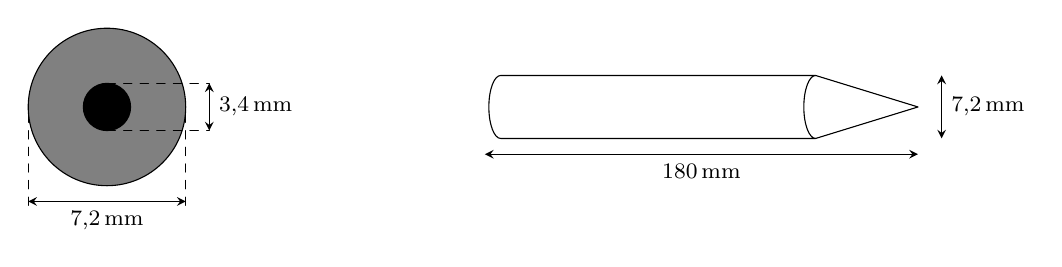
\begin{tikzpicture}[scale=1, font=\footnotesize, line join=round, line cap=round, >=stealth]
			\draw[fill=gray] (-5,0) circle (1);
			\draw[fill=black](-5,0) circle (0.3);
			\filldraw[white,draw=black] (0,0)++(90:0.4) arc (90:270:0.15 and 0.4)--++(0:4) arc (-90:-270:0.15 and 0.4)--cycle;
			\draw[dashed](-6.0,-1.25)--(-6.0,.03);
			\draw[dashed](-4.0,-1.25)--(-4.0,.03);
			\draw[dashed](-5,-0.3)--(-3.7,-0.3);
			\draw[dashed](-5,0.3)--(-3.7,0.3);
			\draw (0,0)++(0:4)++(90:0.4)--(5.3,0)--(4,-0.4);
			\draw[<->] (-3.7,-0.3) --node[midway,right]{3,4\,mm} (-3.7,0.3);
			\draw[<->] (-6,-1.2) --node[midway,below]{7,2\,mm} (-4,-1.2);
			\draw[<->] (-0.2,-0.6) --node[midway,below]{180\,mm} (5.3,-0.6);
			\draw[<->] (5.6,0.4) --node[midway,right]{7,2\,mm} (5.6,-0.4);
		\end{tikzpicture}
	\end{center}
	\begin{enumerate}
		\item Hãy tính thể tích chì cần dùng để làm lõi một cây bút chì khi chưa gọt.
		\item Để có được phần vỏ gỗ của bút chì, người ta dùng những thanh gỗ hình hộp có đáy là hình vuông cạnh $8$\,mm và chiều dài $185$\,mm. Hỏi với $10$\,m$^3$ gỗ chuyên dụng làm vỏ bút chì thì có thể tạo ra được bao nhiêu cây bút chì, biết rằng khi xẻ nhỏ gỗ thì phần hao hụt sẽ chiếm $12\%$ do mùn cưa, gãy, gỗ lỗi, \ldots\\
		Biết công thức tính thể tích hình trụ $V=\pi R^2h$ ($R$ là bán kính đáy, $h$ là chiều cao).
	\end{enumerate}
	\loigiai{
		\begin{enumerate}
			\item Bán kính ruột bút chì hình trụ là $R=\dfrac{3{,}4}{2}=1{,}7$\,(mm).\\
			Thể tích chì cần dùng để làm lõi một cây bút chì khi chưa gọt là 
			$$V=\pi R^2h=\pi\cdot1{,}7^2\cdot180=520{,}2\pi\approx1\,634{,}26\textrm{ (mm$^3$)}.$$
			\item Thể tích gỗ dùng để làm một vỏ bút chì là $V_1={8^2}\cdot185=11\,840$\,(mm$^3$).\\
			Ta có $10$\,m$^3=10\cdot{10}^{9}$\,mm$^3={10}^{10}$\,mm$^3$.\\
			Số vỏ cây bút chì có thể làm ra được từ $10$\,m$^3$ gỗ sau khi trừ đi hao hụt là
			$$\dfrac{10^{10}}{11\,840}\cdot(1-12\%)=743\,243{,}2~(\text{vỏ bút chì}).$$
			Vậy với $10$\,m$^3$ gỗ có thể làm được $743\,243$ vỏ bút chì thỏa mãn yêu cầu.
		\end{enumerate}
	}
\end{bt} 


\subsection{Luyện tập}

\begin{bt}%[Dự án EX-9-Đề Cương Toán 9]%[Đặng Thị Lâm]%[9H4H1-1]
	Cho biết độ dài bán kính đáy và chiều cao của mỗi hình trụ sau.
	\begin{center}
		\begin{tikzpicture}[>=stealth,line join=round,line cap=round,font=\footnotesize,scale=1]
			\def\a{1.4} % ban truc lon = ban kinh tru
			\def\b{0.5} % ban truc nho
			\def\h{2.6} % chieu cao tru
			\path 
			(\a,\h) coordinate (A)
			(\a,0) coordinate (B)
			(0,\h) coordinate (O')
			(0,0) coordinate (O);
			% ve cac canh ben
			\draw (\a,0)--(\a,\h) (-\a,0)--(-\a,\h) (O')--(A);
			\fill (O') circle(1pt);
			\fill (A) circle(1pt);
			% ve day duoi
			\draw[dashed] (\a,0) arc [x radius=\a, y radius=\b, start angle=0, end angle=180];
			\draw (-\a,0) arc [x radius=\a, y radius=\b, start angle=180, end angle=360];
			\draw (0,\h) ellipse (\a cm and \b cm);
			\fill (-\a,0)--(-\a,\h) node[midway,left]{$13$ cm};
			\fill (0.65,2.5) node[above]{$7$ cm};
			\fill (0,-0.5) node[below]{a)};
			\begin{scope}[shift=({3,0})]
				\draw (5,0)--(0,0)--(0,1.2)--(5,1.2);
				\draw (0,0.6) ellipse (0.33 cm and 0.6 cm);
				\draw (5,0) arc [x radius=0.33, y radius=0.6, start angle=-90, end angle=90];
				\draw[dashed] (5,1.2) arc [x radius=0.33, y radius=0.6, start angle=90, end angle=270];
				\draw[<->] (-0.5,0)--(-0.5,1.2) node[midway,above,rotate=90]{$1$ m};
				\fill (2.5,0) node[below]{$4$ m};
				\fill (2.5,-0.5) node[below]{b)};
				%\fill (2.5,-0.98) node[below]{\textit{Hình 2}};
			\end{scope}
			\begin{scope}[shift=({12,0}),rotate=60]
				\draw (0.7,2.6)--(0,2.6)--(0,0) (1.4,0)--(1.4,2.6);
				\draw (0.7,2.6) ellipse (0.7 cm and 0.36 cm);
				\draw (0,0) arc [x radius=0.7, y radius=0.36, start angle=180, end angle=360];
				\draw[dashed] (1.4,0) arc [x radius=0.7, y radius=0.36, start angle=0, end angle=180];
				\fill (0.7,2.6) circle(1pt);
				\fill (0,2.6)--(0,0) node[midway,below,rotate=-30]{$63$ mm};
				\fill (0.35,2.9) node[above,rotate=60]{$16$ mm};
			\end{scope}
			\fill (11.2,-0.5) node[below]{c)};
		\end{tikzpicture}
	\end{center}
	\loigiai{
		Hình trụ ở Hình a) có bán kính đáy $7$ cm, chiều cao $13$ cm;\\
		Hình trụ ở Hình b) có bán kính đáy $0{,}5$ m, chiều cao $4$ m;\\
		Hình trụ ở Hình c) có bán kính đáy $16$ mm, chiều cao $63$ mm.
	}
\end{bt}

%%=====Ví dụ 2
\begin{bt}%[Dự án EX-9-Đề Cương Toán 9]%[Đặng Thị Lâm]%[9H4H1-1]
	Cho hình trụ có chiều cao $15$ cm, bán kính đáy $7$ cm (Hình a) và hình khai triển của hình trụ đó (Hình b). Hãy viết số thích hợp vào mỗi dấu ? trong hình vẽ.
	\begin{center}
		\begin{tikzpicture}[>=stealth,line join=round,line cap=round,font=\footnotesize,scale=1]
			\def\a{1.1} % ban truc lon = ban kinh tru
			\def\b{0.5} % ban truc nho
			\def\h{2.2} % chieu cao tru
			\path 
			(\a,\h) coordinate (A)
			(\a,0) coordinate (B)
			(0,\h) coordinate (O')
			(0,0) coordinate (O);
			% ve cac canh ben
			\draw (\a,0)--(\a,\h) (-\a,0)--(-\a,\h);
			\draw[dashed] (O)--(O') node[midway,right]{$15$ cm};
			\draw[dashed] (O)--(B);
			\fill (O') circle(1pt);
			\fill (O) circle(1pt);
			% ve day duoi
			\draw[dashed] (\a,0) arc [x radius=\a, y radius=\b, start angle=0, end angle=180];
			\draw (-\a,0) arc [x radius=\a, y radius=\b, start angle=180, end angle=360];
			\draw (0,\h) ellipse (\a cm and \b cm);
			\fill (0.55,-0.1) node[above]{$7$ cm};
			\fill (0,-0.65) node[below]{a)};
			\begin{scope}[shift=({3,0})]
				\draw (6,0)--(0,0)--(0,2.2)--(6,2.2)--cycle;
				\draw (1.1,3.3) ellipse (1.1 cm and 1.1 cm);
				\draw (4.9,-1.1) ellipse (1.1 cm and 1.1 cm);
				\draw[dashed] (0,3.3)--(1.1,3.3) (4.9,-1.1)--(6,-1.1);
				\fill (6,0)--(6,2.2) node[midway,right]{? cm};
				\fill (1.1,3.3) circle(1pt);
				\fill (4.9,-1.1) circle(1pt);
				\fill (0.55,3.2) node[above]{? cm};
				\fill (5.45,-1.2) node[above]{? cm};
				\fill (3,-0.7) node[below]{b)};
			\end{scope}
			%\fill (4,-1.6) node[below]{\textit{Hình 3}};
		\end{tikzpicture}
	\end{center}
	\loigiai{
		\begin{center}
			\begin{tikzpicture}[>=stealth,line join=round,line cap=round,font=\footnotesize,scale=1]
				\def\a{1.1} % ban truc lon = ban kinh tru
				\def\b{0.5} % ban truc nho
				\def\h{2.2} % chieu cao tru
				\path 
				(\a,\h) coordinate (A)
				(\a,0) coordinate (B)
				(0,\h) coordinate (O')
				(0,0) coordinate (O);
				% ve cac canh ben
				\draw (\a,0)--(\a,\h) (-\a,0)--(-\a,\h);
				\draw[dashed] (O)--(O') node[midway,right]{$15$ cm};
				\draw[dashed] (O)--(B);
				\fill (O') circle(1pt);
				\fill (O) circle(1pt);
				% ve day duoi
				\draw[dashed] (\a,0) arc [x radius=\a, y radius=\b, start angle=0, end angle=180];
				\draw (-\a,0) arc [x radius=\a, y radius=\b, start angle=180, end angle=360];
				\draw (0,\h) ellipse (\a cm and \b cm);
				\fill (0.55,-0.1) node[above]{$7$ cm};
				\fill (0,-0.65) node[below]{a)};
				\begin{scope}[shift=({3,0})]
					\draw (6,0)--(0,0)--(0,2.2)--(6,2.2)--cycle;
					\draw (1.1,3.3) ellipse (1.1 cm and 1.1 cm);
					\draw (4.9,-1.1) ellipse (1.1 cm and 1.1 cm);
					\draw[dashed] (0,3.3)--(1.1,3.3) (4.9,-1.1)--(6,-1.1);
					\fill (1.1,3.3) circle(1pt);
					\fill (4.9,-1.1) circle(1pt);
					\fill (6,0)--(6,2.2) node[midway,right]{$15$ cm};
					\fill (0.55,3.2) node[above]{$7$ cm};
					\fill (5.45,-1.2) node[above]{$7$ cm};
					\fill (3,-0.7) node[below]{b)};
				\end{scope}
				%\fill (4,-1.6) node[below]{\textit{Hình 4}};
			\end{tikzpicture}
		\end{center}
	}
\end{bt}

\begin{bt}%[Dự án EX-9-Đề Cương Toán 9]%[Đặng Thị Lâm]%[9H4H1-3]
	Tính diện tích xung quanh, diện tích toàn phần và thể tích của hình trụ có
	bán kính đáy $r=8$ cm và chiều cao $h=15$ cm.
	\loigiai{
		\begin{enumerate}
			\item Diện tích xung quanh của hình trụ là $S_{\text{xq}}=2\pi rh=2\pi\cdot8\cdot15=240\pi$ (cm$^2$).
			\item Diện tích toàn phần của hình trụ là
			$$S_{\text{tp}}=2\pi r(r+h)=2\pi\cdot8\cdot(8+15)=368\pi\text{ (cm$^2$)}.$$
			\item Thể tích của hình trụ là $V=\pi r^2h=\pi\cdot8^2\cdot15=960\pi$ (cm$^3$).
		\end{enumerate}
	}
\end{bt}

\begin{bt}%[Dự án EX-9-Đề Cương Toán 9]%[Đặng Thị Lâm]%[9H4V1-4]
	Một hộp kim loại dạng hình trụ có bán kính đáy $4$ cm, chiều cao $10$ cm.
	\begin{enumerate}
		\item Tính diện tích toàn phần của chiếc hộp.
		\item Người ta muốn sơn phần bên ngoài của chiếc hộp kể cả đáy nhưng không sơn nắp hộp. Hỏi diện tích cần sơn là bao nhiêu?
		\item Tính tỉ số phần trăm của diện tích cần sơn và diện tích toàn phần của chiếc hộp.
	\end{enumerate}
	\loigiai{
		\begin{enumerate}
			\item Diện tích xung quanh của chiếc hộp là $S_{\text{xq}}=2\pi rh=2\pi\cdot4\cdot10=80\pi$ (cm$^2$).\\
			Diện tích một đáy của chiếc hộp là $S_{\text{đáy}}=\pi r^2=\pi\cdot4^2=16\pi$ (cm$^2$).\\
			Diện tích toàn phần của chiếc hộp là $S_{\text{tp}}=S_{\text{xq}}+2S_{\text{đáy}}=80\pi+2\cdot16\pi=112\pi$ (cm$^2$).
			\item Diện tích cần sơn là
			$S_{\text{sơn}}=S_{\text{xq}}+S_{\text{đáy}}=80\pi+16\pi=96\pi$. (cm$^2$).
			\item Tỉ số phần trăm của diện tích cần sơn và diện tích toàn phần là $\dfrac{96\pi}{112\pi}\approx85{,}7\%$.
		\end{enumerate}
	}
\end{bt}

\begin{bt}%[Dự án EX-9-Đề Cương Toán 9]%[Đặng Thị Lâm]%[9H4V1-4]
	Người ta khoan một cái lỗ hình trụ có bán kính đáy $4$ cm dọc theo trục của
	một khối gỗ hình trụ có bán kính đáy $10$ cm, chiều cao $12$ cm. Tính thể tích của khối gỗ còn lại (\textit{kết quả làm tròn đến hàng đơn vị của centimét khối}).
	\loigiai{
		Thể tích của khối gỗ hình trụ là $V=\pi r^2h=\pi\cdot10^2\cdot12=1\,200\pi$ (cm$^3$).\\
		Thể tích của cái lỗ hình trụ là $V'=\pi r'^2h=\pi\cdot4^2\cdot12=192\pi$ (cm$^3$).\\
		Thể tích của khối gỗ còn lại là $V-V'=1\,200\pi-192\pi=1\,008\pi\approx3\,167$ (cm$^3$).
	}
\end{bt}